% Options for packages loaded elsewhere
\PassOptionsToPackage{unicode}{hyperref}
\PassOptionsToPackage{hyphens}{url}
\PassOptionsToPackage{dvipsnames,svgnames,x11names}{xcolor}
%
\documentclass[
  letterpaper,
  DIV=11,
  numbers=noendperiod]{scrreprt}

\usepackage{amsmath,amssymb}
\usepackage{iftex}
\ifPDFTeX
  \usepackage[T1]{fontenc}
  \usepackage[utf8]{inputenc}
  \usepackage{textcomp} % provide euro and other symbols
\else % if luatex or xetex
  \usepackage{unicode-math}
  \defaultfontfeatures{Scale=MatchLowercase}
  \defaultfontfeatures[\rmfamily]{Ligatures=TeX,Scale=1}
\fi
\usepackage{lmodern}
\ifPDFTeX\else  
    % xetex/luatex font selection
\fi
% Use upquote if available, for straight quotes in verbatim environments
\IfFileExists{upquote.sty}{\usepackage{upquote}}{}
\IfFileExists{microtype.sty}{% use microtype if available
  \usepackage[]{microtype}
  \UseMicrotypeSet[protrusion]{basicmath} % disable protrusion for tt fonts
}{}
\makeatletter
\@ifundefined{KOMAClassName}{% if non-KOMA class
  \IfFileExists{parskip.sty}{%
    \usepackage{parskip}
  }{% else
    \setlength{\parindent}{0pt}
    \setlength{\parskip}{6pt plus 2pt minus 1pt}}
}{% if KOMA class
  \KOMAoptions{parskip=half}}
\makeatother
\usepackage{xcolor}
\setlength{\emergencystretch}{3em} % prevent overfull lines
\setcounter{secnumdepth}{5}
% Make \paragraph and \subparagraph free-standing
\makeatletter
\ifx\paragraph\undefined\else
  \let\oldparagraph\paragraph
  \renewcommand{\paragraph}{
    \@ifstar
      \xxxParagraphStar
      \xxxParagraphNoStar
  }
  \newcommand{\xxxParagraphStar}[1]{\oldparagraph*{#1}\mbox{}}
  \newcommand{\xxxParagraphNoStar}[1]{\oldparagraph{#1}\mbox{}}
\fi
\ifx\subparagraph\undefined\else
  \let\oldsubparagraph\subparagraph
  \renewcommand{\subparagraph}{
    \@ifstar
      \xxxSubParagraphStar
      \xxxSubParagraphNoStar
  }
  \newcommand{\xxxSubParagraphStar}[1]{\oldsubparagraph*{#1}\mbox{}}
  \newcommand{\xxxSubParagraphNoStar}[1]{\oldsubparagraph{#1}\mbox{}}
\fi
\makeatother

\usepackage{color}
\usepackage{fancyvrb}
\newcommand{\VerbBar}{|}
\newcommand{\VERB}{\Verb[commandchars=\\\{\}]}
\DefineVerbatimEnvironment{Highlighting}{Verbatim}{commandchars=\\\{\}}
% Add ',fontsize=\small' for more characters per line
\usepackage{framed}
\definecolor{shadecolor}{RGB}{241,243,245}
\newenvironment{Shaded}{\begin{snugshade}}{\end{snugshade}}
\newcommand{\AlertTok}[1]{\textcolor[rgb]{0.68,0.00,0.00}{#1}}
\newcommand{\AnnotationTok}[1]{\textcolor[rgb]{0.37,0.37,0.37}{#1}}
\newcommand{\AttributeTok}[1]{\textcolor[rgb]{0.40,0.45,0.13}{#1}}
\newcommand{\BaseNTok}[1]{\textcolor[rgb]{0.68,0.00,0.00}{#1}}
\newcommand{\BuiltInTok}[1]{\textcolor[rgb]{0.00,0.23,0.31}{#1}}
\newcommand{\CharTok}[1]{\textcolor[rgb]{0.13,0.47,0.30}{#1}}
\newcommand{\CommentTok}[1]{\textcolor[rgb]{0.37,0.37,0.37}{#1}}
\newcommand{\CommentVarTok}[1]{\textcolor[rgb]{0.37,0.37,0.37}{\textit{#1}}}
\newcommand{\ConstantTok}[1]{\textcolor[rgb]{0.56,0.35,0.01}{#1}}
\newcommand{\ControlFlowTok}[1]{\textcolor[rgb]{0.00,0.23,0.31}{\textbf{#1}}}
\newcommand{\DataTypeTok}[1]{\textcolor[rgb]{0.68,0.00,0.00}{#1}}
\newcommand{\DecValTok}[1]{\textcolor[rgb]{0.68,0.00,0.00}{#1}}
\newcommand{\DocumentationTok}[1]{\textcolor[rgb]{0.37,0.37,0.37}{\textit{#1}}}
\newcommand{\ErrorTok}[1]{\textcolor[rgb]{0.68,0.00,0.00}{#1}}
\newcommand{\ExtensionTok}[1]{\textcolor[rgb]{0.00,0.23,0.31}{#1}}
\newcommand{\FloatTok}[1]{\textcolor[rgb]{0.68,0.00,0.00}{#1}}
\newcommand{\FunctionTok}[1]{\textcolor[rgb]{0.28,0.35,0.67}{#1}}
\newcommand{\ImportTok}[1]{\textcolor[rgb]{0.00,0.46,0.62}{#1}}
\newcommand{\InformationTok}[1]{\textcolor[rgb]{0.37,0.37,0.37}{#1}}
\newcommand{\KeywordTok}[1]{\textcolor[rgb]{0.00,0.23,0.31}{\textbf{#1}}}
\newcommand{\NormalTok}[1]{\textcolor[rgb]{0.00,0.23,0.31}{#1}}
\newcommand{\OperatorTok}[1]{\textcolor[rgb]{0.37,0.37,0.37}{#1}}
\newcommand{\OtherTok}[1]{\textcolor[rgb]{0.00,0.23,0.31}{#1}}
\newcommand{\PreprocessorTok}[1]{\textcolor[rgb]{0.68,0.00,0.00}{#1}}
\newcommand{\RegionMarkerTok}[1]{\textcolor[rgb]{0.00,0.23,0.31}{#1}}
\newcommand{\SpecialCharTok}[1]{\textcolor[rgb]{0.37,0.37,0.37}{#1}}
\newcommand{\SpecialStringTok}[1]{\textcolor[rgb]{0.13,0.47,0.30}{#1}}
\newcommand{\StringTok}[1]{\textcolor[rgb]{0.13,0.47,0.30}{#1}}
\newcommand{\VariableTok}[1]{\textcolor[rgb]{0.07,0.07,0.07}{#1}}
\newcommand{\VerbatimStringTok}[1]{\textcolor[rgb]{0.13,0.47,0.30}{#1}}
\newcommand{\WarningTok}[1]{\textcolor[rgb]{0.37,0.37,0.37}{\textit{#1}}}

\providecommand{\tightlist}{%
  \setlength{\itemsep}{0pt}\setlength{\parskip}{0pt}}\usepackage{longtable,booktabs,array}
\usepackage{calc} % for calculating minipage widths
% Correct order of tables after \paragraph or \subparagraph
\usepackage{etoolbox}
\makeatletter
\patchcmd\longtable{\par}{\if@noskipsec\mbox{}\fi\par}{}{}
\makeatother
% Allow footnotes in longtable head/foot
\IfFileExists{footnotehyper.sty}{\usepackage{footnotehyper}}{\usepackage{footnote}}
\makesavenoteenv{longtable}
\usepackage{graphicx}
\makeatletter
\newsavebox\pandoc@box
\newcommand*\pandocbounded[1]{% scales image to fit in text height/width
  \sbox\pandoc@box{#1}%
  \Gscale@div\@tempa{\textheight}{\dimexpr\ht\pandoc@box+\dp\pandoc@box\relax}%
  \Gscale@div\@tempb{\linewidth}{\wd\pandoc@box}%
  \ifdim\@tempb\p@<\@tempa\p@\let\@tempa\@tempb\fi% select the smaller of both
  \ifdim\@tempa\p@<\p@\scalebox{\@tempa}{\usebox\pandoc@box}%
  \else\usebox{\pandoc@box}%
  \fi%
}
% Set default figure placement to htbp
\def\fps@figure{htbp}
\makeatother

\KOMAoption{captions}{tableheading}
\makeatletter
\@ifpackageloaded{bookmark}{}{\usepackage{bookmark}}
\makeatother
\makeatletter
\@ifpackageloaded{caption}{}{\usepackage{caption}}
\AtBeginDocument{%
\ifdefined\contentsname
  \renewcommand*\contentsname{Índice}
\else
  \newcommand\contentsname{Índice}
\fi
\ifdefined\listfigurename
  \renewcommand*\listfigurename{Lista de Figuras}
\else
  \newcommand\listfigurename{Lista de Figuras}
\fi
\ifdefined\listtablename
  \renewcommand*\listtablename{Lista de Tabelas}
\else
  \newcommand\listtablename{Lista de Tabelas}
\fi
\ifdefined\figurename
  \renewcommand*\figurename{Figura}
\else
  \newcommand\figurename{Figura}
\fi
\ifdefined\tablename
  \renewcommand*\tablename{Tabela}
\else
  \newcommand\tablename{Tabela}
\fi
}
\@ifpackageloaded{float}{}{\usepackage{float}}
\floatstyle{ruled}
\@ifundefined{c@chapter}{\newfloat{codelisting}{h}{lop}}{\newfloat{codelisting}{h}{lop}[chapter]}
\floatname{codelisting}{Listagem}
\newcommand*\listoflistings{\listof{codelisting}{Lista de Listagens}}
\makeatother
\makeatletter
\makeatother
\makeatletter
\@ifpackageloaded{caption}{}{\usepackage{caption}}
\@ifpackageloaded{subcaption}{}{\usepackage{subcaption}}
\makeatother

\ifLuaTeX
\usepackage[bidi=basic]{babel}
\else
\usepackage[bidi=default]{babel}
\fi
\babelprovide[main,import]{portuguese}
% get rid of language-specific shorthands (see #6817):
\let\LanguageShortHands\languageshorthands
\def\languageshorthands#1{}
\usepackage[]{biblatex}
\addbibresource{references.bib}
\usepackage{bookmark}

\IfFileExists{xurl.sty}{\usepackage{xurl}}{} % add URL line breaks if available
\urlstyle{same} % disable monospaced font for URLs
\hypersetup{
  pdftitle={Anotaçõess de Inferência Frequentista},
  pdfauthor={Gustavo S. Garone},
  pdflang={pt},
  colorlinks=true,
  linkcolor={blue},
  filecolor={Maroon},
  citecolor={Blue},
  urlcolor={Blue},
  pdfcreator={LaTeX via pandoc}}


\title{Anotaçõess de Inferência Frequentista}
\author{Gustavo S. Garone}
\date{2025-02-01}

\begin{document}
\maketitle

\renewcommand*\contentsname{Índice}
{
\hypersetup{linkcolor=}
\setcounter{tocdepth}{2}
\tableofcontents
}

\bookmarksetup{startatroot}

\chapter*{Preface}\label{preface}
\addcontentsline{toc}{chapter}{Preface}

\markboth{Preface}{Preface}

This is a Quarto book.

To learn more about Quarto books visit
\url{https://quarto.org/docs/books}.

\bookmarksetup{startatroot}

\chapter{Introdução}\label{introduuxe7uxe3o}

Este livrete é um compilado de minhas anotações para as Disciplinas
MAE0225 e MAE301, ambas ministradas pelo Professor Alexandre Galvão
Patriota.

Para quaisquer erros, sugestões e críticas, contactar em
\href{gustavo.garone@usp.br}{gustavo.garone arroba usp.br}

\bookmarksetup{startatroot}

\chapter{Modelos Estatísticos na abordagem
clássica}\label{modelos-estatuxedsticos-na-abordagem-cluxe1ssica}

Em teoria de probabilidades, conhecemos a medida de probabilidade, logo,
fazemos descrições probabilísticas.
\[(\Omega, \mathscr{A}, P)\stackrel{\text{X}}{\rightarrow}(\mathbb{R}, \mathscr{B}, P_{X})\]
Na prática, contudo, não conhecemos a medida \(P\).

Definimos então uma família de medidas de probabilidades que
possivelmente descrevem o comportamento aleatório dos dados.

O \emph{Modelo Estatístico} é definido pela trinca
\[(\Omega, \mathscr{A}, \mathscr{P})\] em que \(\Omega\) é o espaço
amostral (evento certo), \(\mathscr{A}\) é a Sigma álgebra, uma família
de subconjuntos ou eventos em \(\Omega\), e \(\mathscr{P}\) é uma
família de medidas de probabilidade que possivelmente descrevem o
comportamento aleatório dos dados ou eventos sobre investigação.

\section{Modelo Estatístico
Paramétrico}\label{modelo-estatuxedstico-paramuxe9trico}

Se \(\mathscr{P} = \{P_{\theta} : \theta \in \Theta\}\), em que
\(\Theta \subseteq \mathbb{R}^{P}\) e \(p \in \mathbb{N}\), então
dizemos que \((\Omega, \mathscr{A}, \mathscr{P})\) é um modelo
estatístico \textbf{Paramétrico}.

Caso não exista \(\Theta \subseteq \mathbb{R}^{P}\) fixo, então dizemos
que o modelo é não-paramétrico. \emph{Obs}: \(\Theta\) é o espaço
paramétrico e \(\theta\) é o vetor de parâmetros. \(\theta\)
\textbf{Não}* é variável aleatória, apenas indexa as medidas de
probabilidade.

\subsection{Exemplos}\label{exemplos}

\subsubsection{Exemplo de Bernoulli}\label{exemplo-de-bernoulli}

Considere um Ensaio de Bernoulli
\[\Omega = \{S,F \}, \mathscr{A} = 2^\Omega\] Temos algum conhecimento
prévio que sugere que as probabilidades de sucesso podem ser
\(0.1, 0.5, 0.9\)

Nesse caso, \[\mathscr{P} = \{P_{1}, P_{2}, P_{3} \}\] em que
\[\begin{cases}
P_{1}(\{S\}) = 0.1;~ P_{1}(\{F\}) = 0.9;~ P_{1}(\Omega) = 1  \\
P_{2}(\{S\}) = 0.5;~ P_{2}(\{F\}) = 0.5;~ P_{2}(\Omega) = 1  \\
P_{3}(\{S\}) = 0.9;~ P_{3}(\{F\}) = 0.1;~ P_{3}(\Omega) = 1 
\end{cases}\] Observe que
\[\mathscr{P}=\{P_{\theta}: \theta \in \Theta \}\] em que
\(\Theta=\{1,2,3 \}\subseteq \mathbb{R}\) Portanto,
\((\Omega, \mathscr{A}, \mathscr{P})\) é um modelo paramétrico.

\subsubsection{Exemplo de Exponencial}\label{exemplo-de-exponencial}

Seja \(X : \Omega \rightarrow \mathbb{R}\) tal que
\[X(\omega)=\begin{cases}
1, \omega = \text{S} \\
0, c.c.
\end{cases}\] \[E_\theta(X)=\sum\limits^{1}_{x=0}xP_\theta(X=x)\]
\[\begin{cases}
\theta = 1 \Rightarrow E_{1}(X)=0.1 \\
\theta = 2 \Rightarrow E_{2}(X)=0.5 \\
\theta = 3 \Rightarrow E_{3}(X)=0.9
\end{cases}\] Seja \(\Omega=(0,\infty)\) e \(\mathscr{A}\) uma
sigma-álgebra de \(\Omega\) (Sigma-Álgebra de Borel) \(\Omega\)
representa o tempo até a ocorrência de um evento (uma reclamação, por
exemplo) Temos conhecimento prévio de que as funções densidade de
probabilidade que possivelmente descrevem esse evento são:

\[
\begin{aligned}
f_{1}(\omega) &=
\begin{cases}
\mathrm{e}^{-1\omega}, \omega>0 \\
0, c.c.
\end{cases}\\
f_{2} (\omega) &=
\begin{cases}
2\mathrm{e}^{-2\omega}, \omega>0 \\
0, c.c.
\end{cases}\\
f_{3} (\omega) &=
\begin{cases}
\frac{1}{2}\mathrm{e}^{-\frac{1}{2}\omega}, \omega>0 \\
0, c.c.
\end{cases}\\
f_{4} (\omega) &=
\begin{cases}
\frac{1}{10}\mathrm{e}^{- \frac{1}{10}\omega}, \omega>0 \\
0, c.c.
\end{cases}
\end{aligned}
\]

e \(P\)s, \[
\begin{aligned}
P_{1}(A)&= \int_{A} f_{1}(\omega)d \omega \\
P_{2}(A)&= \int_{A} f_{2}(\omega)d \omega \\
P_{3}(A)&= \int_{A} f_{3}(\omega)d \omega \\
P_{4}(A)&= \int_{A} f_{4}(\omega)d \omega \\
\end{aligned}\] Dessa forma,
\[P_{\theta}= \int_{A}f_\theta(\omega)d \omega, \omega \in \Omega\] e
\(\Omega = \{1,2,3,4 \}\) Seja \(X: \Omega \rightarrow \mathbb{R}\) tal
que \[X(\omega)= \omega\] Note que
\[E_\theta(X)=\int_{-\infty}^{\infty}xf_\theta(x)dx, \theta \in \{1,2,3,4 \}\]
\[E_\theta(X)=\begin{cases}
1,~ \theta=1 \\
\frac{1}{2},~ \theta=2 \\
2,~ \theta=3 \\
10,~ \theta=4
\end{cases}
\]

\section{Principais Modelos
Estatísticos}\label{principais-modelos-estatuxedsticos}

\subsection{Modelo Estatístico de Bernoulli}\label{sec-modelobernoulli}

Dizemos que X é uma variável aleatória com modelo de Bernoulli se, e
somente se, \[
P_\theta(X=x)=\begin{cases}
\theta^{x} \cdot(1-\theta)^{1-x}, x \in \{0,1 \} \\
0, x \not \in \{0,1 \}
\end{cases}\] em que \(\theta \in \Theta\) e
\(\Theta=(0,1)\subseteq \mathbb{R}\) O parâmetro é a probabilidade de
sucesso \[\begin{cases}
E_\theta(X)=\theta\\
\mathrm{Var}_{\theta}(X) = \theta(1-\theta) \\
P_\theta(X=1)=\theta, P_\theta(X=0)=1-\theta
\end{cases}
\]

\subsection{Modelo Estatístico
Binomial}\label{modelo-estatuxedstico-binomial}

Dizemos que \(X\) é uma variável aleatória com modelo binomial se, e
somente se, \[
P_\theta(X=x)=\begin{cases}
{n \choose x} \cdot \theta^{x}\cdot(1-\theta)^{n-x}, x \in \{0,1,\dots,n \} \\
0, x \not \in \{0,1,\dots,n \}
\end{cases}\] em que \(n\) é conhecido e fixado previamente, \(\theta\)
é a probabilidade de sucesso (parâmetro do modelo) e \(\Theta =(0,1)\) é
o espaço paramétrico \[\begin{cases}
E_\theta(X)=n\theta\\
\mathrm{Var}_{\theta}(X) = n\theta(1-\theta) \\
P_\theta(X=0)=(1-\theta)^{n},\dots, P_\theta(X=n)=\theta^n
\end{cases}\]

\subsection{Modelo Estatístico
Geométrico}\label{modelo-estatuxedstico-geomuxe9trico}

Dizemos que \(X\) é uma variável aleatória com modelo estatístico
geométrico se, e somente se, \[P_\theta(X=x)=\begin{cases}
\theta (1-\theta)^{x-1}, x \in \{1,\dots\} \\
0, x \not \in \{1,\dots\}
\end{cases}
\] em que \(\theta\) é o parâmetro do modelo (probabilidade de sucesso)
e \(\Theta=(0,1)\) é o espaço paramétrico \[
\begin{cases}
E_\theta(X)=\frac{1}{\theta}\\
\mathrm{Var}_\theta(X) = \frac{1-\theta}{\theta^{2}}
\end{cases}
\]

\subsection{Modelo de Poisson}\label{modelo-de-poisson}

Dizemos que \(X\) é uma variável aleatória com modelo estatístico
Poisson, se, e somente se, \[
P_\theta(X=x)=\begin{cases}
\mathrm{e}^{-\theta}\cdot \frac{\theta^{x}}{x!}, x \in \{0,1,\dots\} \\
0, x \not \in \{0,1,\dots\}
\end{cases}
\] em que \(\theta\) é a taxa média de ocorrência do evento (parâmetro
do modelo) e \(\Theta = (0, \infty)\), o espaço paramétrico. \[
\begin{cases}
E_\theta(X)=\theta\\
\mathrm{Var}_\theta(X) = \theta
\end{cases}
\]

\subsection{Modelo Multinomial}\label{modelo-multinomial}

Dizemos que \(X\) é um Vetor Aleatório com modelo estatístico
Multinomial se, e somente se a função de probabilidade é \[
P_{\theta}(X_{1}=x_{1},\dots,X_{k} = x_{k})=\begin{cases}
\frac{n!}{x_{1}!x_{2}!\dots x_{k}!} \cdot \theta^{x_{1}}_{1} \cdot,\cdots, \cdot\theta^{x_n}_{k} ~~~~ x_{1}+\dots+x_{k}=n\\
0, c.c
\end{cases}
\]

em que \(\theta_{1}+\dots+\theta_{k}=1\) e \(0\leq \theta_{i} \leq 1\),
\(\forall i = 1,2,\dots,k\),
\(\Theta=\{(\theta_{1},,\dots,\theta_{k}) \in \mathbb{R}^{k} : 0\leq \theta_{i} \leq 1, i=1,\dots,k,
\theta_{1}+\dots+\theta_{k} = 1 \}\)

\[
\begin{cases}
E_\theta(X_{i})=n\theta_{i}\\
\mathrm{Var}_\theta(X_{i}) = n\theta_{}i (1-\theta_{i}) \\
\mathrm{Cov}(X_{i}X_{j})=-n\theta_{i}\theta_{j}
\end{cases}
\] Esse modelo tem aplicação em modelos de linguagem como o ChatGPT.
(\(k\) como tamanho do vocabulário, \(n=1\), \(\theta_{1}=\)
probabilidade de escolher o primeiro elemento do vocabulário e assim por
diante.)

\subsection{Modelo Uniforme contínuo}\label{modelo-uniforme-contuxednuo}

Dizemos que \(X\) é uma variável aleatória contínua com modelo
estatístico Uniforme em
\((\theta_{1}, \theta_{2}), \theta_{2}>\theta_{1}\), se, e somente se, a
sua Função Densidade de Probabilidade é \[
f_\theta(x)=\begin{cases}
\frac{1}{\theta_{2}-\theta_{1}}, x \in(\theta_{1}, \theta_{2}) \\
0, c.c.
\end{cases}
\] em que \(\theta=(\theta_{1}, \theta_{2})\) vetor,
\(\Theta = \{\theta \in \mathbb{R}^{2} : \theta_{2} > \theta_{1} \}\)

\[
\begin{cases}
E_\theta(X)=\frac{b+a}{2}\\
\mathrm{Var}_\theta(X) = \frac{(b-a)^{2}}{12}\end{cases}
\]

\[
X \sim U(\theta_{1}, \theta_{2}), \theta=(\theta_{1}, \theta_{2}) \text{ Vetor de Parâmetros}
\]

\subsection{Modelo Exponencial}\label{modelo-exponencial}

Dizemos que \(X\) é uma variável aleatória contínua com modelo
estatístico Exponencial se, e somente se, a sua Função Densidade de
Probabilidade é dada por \[
f_\theta(x)=\begin{cases}
\theta \mathrm{e}^{-\theta x}, x>0\\
0, c.c.
\end{cases}
\]

em que \(\theta>0, \Theta=\{\theta \in \mathbb{R}: \theta>0 \}\)

\[
\begin{cases}
E_\theta(X)=\frac{1}{\theta}\\
\mathrm{Var}_\theta(X) = \frac{1}{\theta^{2}}
\end{cases}
\]

\[
X\sim \mathrm{Exp}(\theta), \theta> 0
\]

\subsection{Modelo Normal}\label{modelo-normal}

Dizemos que \(X\) é uma variável aleatória contínua com modelo
estatístico Normal com média \(\mu\) e variância \(\sigma^{2}\) se, e
somente se, a sua Função Densidade de Probabilidade é dada por

\[
f_\theta(x)=
\frac{1}{\sqrt{2\pi \sigma^{2}}}\cdot \mathrm{e}^{-\frac{1}{2\sigma^{2}}(x-\mu)^{2}}, x \in \mathbb{R}
\] em que
\(\theta= (\mu, \sigma^{2}) \in \Theta=\{(\mu, \sigma^{2}) \in \mathbb{R}\times \mathbb{R}^{+}\}\)

\[
\begin{cases}
E_\theta(X)=\mu\\
\mathrm{Var}_\theta(X) = \sigma^{2}
\end{cases}
\]

\[
X \sim N (\mu, \sigma^{2}), \theta=(\mu, \sigma^{2}) \text{ Vetor de Parâmetros}
\]

\bookmarksetup{startatroot}

\chapter{População e Amostra}\label{populauxe7uxe3o-e-amostra}

Veja: \href{modelo-estatistico.qmd}{Modelo Estatístico} para definições
dos modelos estatísticos paramétricos.

\section{Variável Populacional}\label{sec-vp}

Pela teoria estatística, população é o conjunto sob investigação de
todos os potenciais elementos.

A \emph{Variável Populacional} representa os valores numéricos de cada
elemento da população: \[
X\sim f_{\theta,}\theta \in \Theta
\] em que \(f_\theta\) é a Função Densidade de Probabilidade da Variável
Aleatória populacional. \(\theta\) é o vetor de parâmetros
(desconhecido) e \(\Theta\) é o espaço paramétrico

\section{Amostra (Teórica)}\label{amostra-teuxf3rica}

É uma parte ou subconjunto da população.

\subsection{Amostra Aleatória}\label{sec-aa}

Dizemos que \((X_{1},\dots,X_{n})\) é uma amostra aleatória de X (v.a.
populacional) se \(X_{1},\dots,X_{n}\) forem independentes e
identicamente distribuídas de acordo com a distribuição de \(X\) Ou
seja, \[
\text{Independentes = }\begin{cases}X_{1}\sim f_{\theta,}\theta \in \Theta \\
. \\
. \\
. \\
X_{n} \sim f_{\theta}, \theta \in \Theta
\end{cases}
\]

\section{Amostra (Observada)}\label{sec-ao}

É formada por valores numéricos após utilizar um procedimento de
amostragem. \[
x_{1},\dots,x_{n}
\]

em que \(n\) é o tamanho amostral.

\bookmarksetup{startatroot}

\chapter{Quantidade de Interesse}\label{quantidade-de-interesse}

É uma quantidade relacionada com a distribuição da
\hyperref[sec-vp]{variável aleatória populacional}. \[
g(\theta)
\]

Como
\(g(\theta) = E_\theta(X), g(\theta)= \mathrm{Var}_\theta(X), g(\theta)=P_\theta(X\geq1)\)
e até \(g(\theta)=\theta\)

\bookmarksetup{startatroot}

\chapter{Distribuição Amostral}\label{distribuiuxe7uxe3o-amostral}

Seja \((X_{1},\dots,X_{n})\) \hyperref[sec-aa]{amostra aleatória (a.a.)}
de \(X\sim f_{\theta,}\theta \in \Theta\)

a Função Densidade de Probabilidade conjunta de
\((X_{1}, X_{2},\dots,X_{n})\) é \(\forall \theta \in \Theta\), no caso
discreto: \[
P_\theta(X_{1}=k_{1}, X_{2}=k_{2},\dots,X_{n}= k_{n})\stackrel{\text{ind}}{=}\prod^{n}_{i=1}P_\theta(X_{i}=k_{i})
\stackrel{\text{id}}{=}\prod^{n}_{i=1}P_\theta(X=k_{i})\stackrel{\text{def}}{=}\prod^{n}_{i=1}f_\theta(k_{i})
\]

no caso contínuo: \[
f_\theta^{(x)}(k_{1},k_{2},\dots,k_{n})\stackrel{\text{i.i.d}}{=}\prod^{n}_{i=1}f_{\theta}(k_{i})
\]

\section{Exemplos}\label{exemplos-1}

\subsection{Exemplo um}\label{exemplo-um}

Seja \((X_{1},X_{2},X_{3})\) uma a.a de
\(X\sim \text{Ber}(\theta), \theta \in (0,1)\) 1. Especifique o espaço
paramétrico 2. Calcule a função de probabilidade da amostra 3. Encontre
as seguintes \href{quantidade-de-interesse.qmd}{quantidade de
interesses} em função de \(\theta\) 1. \(g(\theta)=E_\theta(X)\) 2.
\(g(\theta)=P_\theta(X=0)\) 3. \(g(\theta)=\mathrm{CV}_\theta(X)\)
Resolução 1. \(\Theta=(0,1)\) 2. Duas resoluções possíveis 1. Dando
valores à amostra \[\begin{aligned}
         &(X_{1}, X_{2},X_{3})  &P(X_{1}= k_{1},X_{2}= k_{2},X_{3}= k_{3})= \prod ^{3}_{i=1}P_\theta(X=k_{1})\\
         &(0,0,0) &(1-\theta)^{3}\\
         &(0,0,1) &(1-\theta)^{2}\theta\\
         &(0,1,0) &(1-\theta)^{2}\theta\\
         &(1,0,0) &(1-\theta)^{2}\theta\\
         &(0,1,1) &(1-\theta)\theta^2\\
         &(1,0,1) &(1-\theta)\theta^{2}\\
         &(1,1,0) &(1-\theta)\theta^{2}\\
         &(1,1,1) &\theta^{3}\\
         \end{aligned}
    \] 2. Enunciando a função Observe que, se \(k \in \{0,1 \}\),
\[\begin{aligned}
       &P_\theta(X=k)=\theta^{k}(1-\theta)^{1-k}\cdot\mathbb{1}_{\{0,1 \}}(k)\Rightarrow\\
       &P_\theta(X_{1}=k,X_{2}=k_{2},X_{3}= k_{3})\stackrel{\text{i.i.d}}{=}\prod^{3}_{i=1}\{\theta^{k_{i}}
       (1-\theta)^{1-k_{1}}\mathbb{1}_{\{0,1 \}}(k_{1}) \} = \\
       &= \theta^{\sum\limits^{3}_{i=1}k_{1}}(1-\theta)^{3-\sum\limits^{3}_{i=1}k_{1}}\prod^{3}_{i=1}\mathbb{1}_{\{0,1\}}
       (k_{i})
       \end{aligned}
    \] 3. Em função de \(\theta\): 1. \(g(\theta)=E_\theta(X)=\theta\)
2. \(g(\theta)=P_\theta(X=0)=1-\theta\) 3.
\(g(\theta)=\mathrm{CV}_\theta(X)=\frac{\sqrt{\theta(1-\theta)}}{\theta}\)

\subsection{Exemplo dois}\label{exemplo-dois}

Seja \((X_{1},\dots,X_{n})\) uma a.a de
\(X\sim\text{Ber}(\theta), \theta \in(0,1)\), encontre a f.p conjunta da
amostra. \[
\begin{aligned}
P_\theta(X_{1}=k_{1},\dots,X_{n}=k_{n})\stackrel{\text{iid}}{=}\prod ^{n}_{i=1}P_\theta(X=k_{i})=\prod^{n}_{i=1}
\{\theta^{k_{i}}(1-\theta)^{1-k_{i}}\mathbb{1}_{\{0,1 \}}(k_{i}) \}\\
\Rightarrow P_\theta(X_{1}=k_{1},\dots,X_{n}=k_{n})=\theta^{\sum\limits^{n}_{i=1}k_{1}}\cdot 
\theta^{n-\sum\limits^{n}_{i=i}k_{i}}\cdot\mathbb{1}_{\{0,1\}}(k_{i})
\end{aligned}
\]

\subsection{Exemplo três}\label{exemplo-truxeas}

Seja \((X_{1},\dots,X_{n})\) uma a.a de
\(X\sim\text{Pois}(\theta), \theta \in(0,\infty)\), encontre a f.p.
conjunta da amostra. Como esse vetor é uma a.a. (ou seja, variáveis
aleatórias independentes e identicamente distribuídas), temos que \[
P_\theta(X_1=k_{1},\dots,X_{n}=k_{n})\stackrel{\text{iid}}{=}\prod^{n}_{i=1}P_\theta(X=k_{i})=\prod^{n}_{i=1}\{\mathrm{e}
^{-\theta} \cdot \frac{\theta^{k_{i}}}{k_{i}!}\}
\] Sempre que \(k_{i}\in\{0,1,\dots \}, \forall i = 1,\dots,n\)

\[
\Rightarrow P_\theta(\dots)=\mathrm{e}^{-n \theta} \cdot \frac{\theta^{\sum\limits^{n}_{i=1}k_{i}}}{\prod^{n}_{i=1}
(k_{i})!}
\]

\subsection{Exemplo contínuo um}\label{exemplo-contuxednuo-um}

Seja \((X_{1},\dots,X_{n})\) uma a.a de
\(X\sim\text{Exp}(\theta), \theta \in(0,\infty)\), encontre a função
densidade de probabilidade (f.d.p.) conjunta da amostra. \[
\begin{aligned}
F_{\theta}^{(*)}(k_{1},\dots,k_{n})&\stackrel{\text{iid}}{=}\prod^{n}_{i=1}f_\theta(k_{i})=\prod^{n}_{i=1}
\{\theta \mathrm{e}^{-\theta k_{i}} \cdot \mathbb{1}_{(0,\infty )}(k_{i}) \}
\\&\Rightarrow f_\theta^{(*)}(\dots)=\theta^{n}
\cdot \mathrm{e}^{-\theta\sum\limits^{n}_{i=1}k_{i}} \cdot\prod^{n}_{i=1}\mathbb{1}_{(0,\infty)}(k)
\end{aligned}
\]

\subsection{Exemplo contínuo dois}\label{exemplo-contuxednuo-dois}

Seja \((X_{1},\dots,X_{n})\) uma a.a. (i.i.d) de
\(X\sim N(\mu,\sigma^{2})\) em que
\(\theta=(\mu, \sigma^{2}) \in \Theta=\mathbb{R}\times \mathbb{R}_{+}\).
Considere \(\stackrel{x}{\sim}=(x_{1},\dots,x_{n})\) a amostra
observada.

\[
\begin{aligned}
L_{\stackrel{X}{\sim}} &\stackrel{\text{iid}}{=} \prod^{n}_{i=1}f_\theta(x_{i})=
\prod^{n}_{i=1}\left\{\frac{1}{\sqrt{2 \pi \sigma^{2}}} \mathrm{exp}\{- \frac{1}{2\sigma^{2}}(x_{1}-\mu)^{2}\}\right\} \\
&= \frac{1}{(2 \pi \sigma^{2})^{\frac{x}{2}}}\cdot \mathrm{exp}\{- \frac{1}{2 \sigma^{2}} \sum\limits^{n}_{i=1}(x_{i}-\mu)^{2}  \}
\end{aligned}
\]

\bookmarksetup{startatroot}

\chapter{Função de
Verossimilhança}\label{funuxe7uxe3o-de-verossimilhanuxe7a}

Quando analisamos a \href{dist-amostral.qmd}{distribuição conjunta da
amostra} em função de \(\theta\) nos valores da
\hyperref[sec-ao]{amostra observada}, temos a \textbf{Função de
Verossimilhança}

\[
\mathrm{L}_{\stackrel{x}{\sim}}(\theta)=P_\theta(X_{1}=x_{1},X_{2}=x_{2},\dots,X_{n}=x_{n})
\]

em que \(\stackrel{x}{\sim}=(x_{1},x_{2},\dots,x_{n})\) é a amostra
observada.

Obs: A função de verossimilhança, no caso discreto, é a probabilidade de
observar a amostra observada.

\section{Exemplo}\label{exemplo}

Considere \((X_{1},X_{2},X_{3},X_{4})\) a.a de
\(X\sim \text{Ber}(\theta), \theta \in \{0.1, 0.5, 0.9 \}\). Note que o
espaço paramétrico é \(\Theta=\{0.1,0.5,0.9 \}\). Considere, ainda, que
a amostra observada foi \((0,1,1,1)\). Encontre a função de
verossimilhança.

\[
\begin{aligned}
L_\stackrel{X}{\sim}(\theta)&=P_\theta(X_{1}=x_{1},X_{2}=x_{2},X_{3}=x_{3},X_{4}=x_{4}) \\
&= \theta^{\sum\limits^{4}_{i=1}x_{i}}
(1-\theta)^{4-\sum\limits^{4}_{i=1}x_{i}}\cdot \cancelto{1}{\prod^{4}_{i=1}\mathbb{1}_{\{0,1 \}}(x_{i})} = 
\theta^{3}(1-\theta)
\end{aligned}
\]

\bookmarksetup{startatroot}

\chapter{Estatísticas}\label{estatuxedsticas}

Funções da \hyperref[sec-aa]{amostra} que não dependem de
\(\theta \in \Theta\)

\section{Exemplo}\label{exemplo-1}

Seja \((X_{1}, \dots, X_{n})\) a.a. de
\(X\sim f_{\theta,}\theta \in \Theta\). São estatísticas: 1.
\(T_{1}(X_{1},\dots,X_{n})=X_{1}+\dots+X_{n}\) 2.
\(T_{2}=\bar{X}= \frac{X_{1}+\dots+X_{n}}{n}\) 3.
\(T_{3}=\max\{X_{1},\dots,X_{n}\}=X_{(n)}\) 4.
\(T_{4}=\min\{X_{1},\dots,X_{n}\}=X_{(1)}\) 5.
\(T_{5}(X_{1},\dots,X_{n})=X_{(n})-X_{(1)}\) 6.
\(T_{6}(X_{1},\dots,X_{n})=X_{i}, \text{para algum }i=1,\dots,n\) 7.
\(T_{7}(X_{1},\dots,X_{n})=\frac{1}{n}\sum\limits^{n}_{i=1}(X_{i}-\bar{X})^{2}\)
8.
\(T_{8}(X_{1},\dots,X_{n})=\frac{1}{n-1}\sum\limits^{n}_{i=1}(X_{i}-\bar{X})^{2}\)
9.
\(T_{9}(X_{1},\dots,X_{n})=\frac{1}{n}\sum\limits^{n}_{i=1}|X_{i}-\bar{X}|\)
10.
\(T_{7}(X_{1},\dots,X_{n})=\sqrt{\frac{1}{n}\sum\limits^{n}_{i=1}(X_{i}-\bar{X})^{2}}\)
etc.

\textbf{Observação:} As estatísticas são variáveis aleatórias.

\[
\underset{\sim}{X_n}=(X_{1},\dots,X_{n}):\Omega\rightarrow \mathbb{R}^{n}
\] \[
T(\underset{\sim}{X})=T \circ \underset{\sim}{X}:\Omega\rightarrow \mathbb{R}
\]

\bookmarksetup{startatroot}

\chapter{Estimadores}\label{estimadores}

São estatísticas cujo objetivo é estimar uma
\href{quantidade-de-interesse.qmd}{quantidade de interesse}. Portanto,
estimadores são também variáveis aleatórias.

\section{Estimativas}\label{estimativas}

São os valores observados a partir da amostra observada dos estimadores.
Portanto, \emph{estimativas são valores numéricos}

Exemplos: 1. \(\bar{X}\) é uma estatística, \(\bar{X}\) é um estimador
para \(g(\theta)=E_\theta(X)\) 2. Observando
\(\bar{x}=\frac{1}{n} \sum\limits^{n}_{i=1}x_{i}\) é uma estimativa Seja
\((X_{1},X_{2})\) a.a de \(X\sim \text{Ber}(\theta), \theta \in (0,1)\).
Considere as estatísticas e suas funções de probabilidade: \[
\begin{aligned}
T_{1}(X_{1},X_{2}) &= X_{1}\\
T_{2}(X_{1},X_{2}) &= X_{2}\\
T_{3}(X_{1},X_{2}) &= X_{1}+X_{2}\\
T_{4}(X_{1},X_{2}) &= \max\{X_{1},X_{2}\}\\
T_{5}(X_{1},X_{2}) &= \min\{X_{1},X_{2}\}\\
T_{6}(X_{1},X_{2}) &= \frac{1}{2}[(X_{1}-\bar{X})^{2}+(X_{2}-\bar{X})^{2}]=S^{2}_{n}=\frac{1}{2}S_{n-1}^{2}
\end{aligned}
\]

\[
\begin{array}{cccccc}
(X_{1},X_{2}) & P_{\theta X_{1},X_{2}} & X_{1} & X_{2} & X_{1}+X_{2} & T_4 & T_5 & \bar{X}& S^{2}_{n} & S^{2}_{n-1}\\
\hline
(0,0) & (1-\theta)^{2} & 0 & 0 & 0 & 0 & 0 & 0 & 0 & 0\\
(1,0) & \theta(1-\theta) & 1 & 0 & 1 & 1 & 0 & 0.5 & 0.25 & 0.5\\
(0,1) & \theta(1-\theta) & 0 & 1 & 1 & 1 & 0 & 0.5 & 0.25 & 0.5\\
(1,1) & \theta^{2} & 1 & 1 & 2 & 1 & 1 & 1 & 0 & 0\\
\hline
\end{array}
\]

Calcule para \(T \in \{T_{1},T_{2},T_{3},T_{4},T_{5},T_{6} \}\)

a-) \(E_\theta(T)\)

\(E_\theta(T_{1}(X_{1},X_{2}))=E_\theta(X_{1})=\theta =0 (1-\theta)^{2}+1 \cdot\theta(1-\theta)+0 \theta(1-\theta)+1
\theta^{2}= \theta\)

O mesmo vale para \(T_2\)

\(E_\theta(T_{3}(X_{1},X_{2}))=E_\theta(X_{1}+X_{2})=2 \theta\)
\(E_\theta(T_{4}(X_{1},X_{2}))=E_\theta(\max\{X_{1},X_{2}\})=0 \cdot (1-\theta)^{2}+ 1\cdot[2\cdot \theta(1-\theta)+
\theta^{2}] = 2\theta-\theta^{2}\)
\(E_{\theta}(T_{5}(X_{1},X_{2}))=E_\theta(\min\{X_{1},X_{2} \})=\theta^{2}\)
\(E_\theta(T_{6}(X_{1},X_{2}))=2 \theta(1-\theta)\)

b-) \(\mathrm{Var}_{\theta}(T)\)

Termine com os mesmos raciocínios

c-) \(P_\theta(T=0)\)

Termine com os mesmos raciocínios

Alguns resultados importantes:

\[
\begin{aligned}
E_\theta(\bar{X})&=E_\Theta(\frac{X_{1}+X_{2}}{2})=\theta, \theta \in(0,1)\\
E_{\theta}(\bar{X}^{2}) &= 0^{2}(1-\theta)^{2} + \frac{2}{4}  \theta (1-\theta) + 1^{2}\theta^{2}=\frac{1}{2}\theta +
\frac{1}{2} \theta^{2}, \theta \in(0,1)\\
\Rightarrow \mathrm{Var}_\theta(\bar{X}) &= \frac{\theta+\theta^{2}}{2} - \theta^{2} =\frac{\theta (1-\theta)}{2}, 
\theta \in(0,1)
\end{aligned}
\]

Aplicando em nossa tabela (\(S_{n-1}^{2}\)):

\[
\begin{aligned}
E_\theta([(X_{1}-\bar{X})^{2}+(X_{2}-\bar{X})^{2}])&= \theta(1-\theta)\\
E_\theta([(X_{1}-\bar{X})^{2}+(X_{2}-\bar{X})^{2}]^{2}) &= \frac{\theta(1-\theta)}{2}\\
\Rightarrow\mathrm{Var}_{\Theta}([(X_{1}-\bar{X})^{2}+(X_{2}-\bar{X})^{2}]) &= \frac{1}{2}\theta(1-\theta)
[1-2 \cdot \theta(1-\theta)]
\end{aligned}
\]

\section{Propriedades dos estimadores para quantidades de
interesse}\label{propriedades-dos-estimadores-para-quantidades-de-interesse}

\subsection{Estimados não viciados ou
enviesados}\label{estimados-nuxe3o-viciados-ou-enviesados}

Seja \((X_{1},\dots,X_{n})\) a.a. de
\(X\sim f_{\theta,}\theta \in \Theta\) e considere
\(T(X_{1},\dots,X_{n})=\hat\theta\) um estimador para \(\theta\).
Dizemos que \(\hat \theta\) é \emph{não-enviesado} para \(\theta\)
\(\Leftrightarrow\) \[
E_\theta(\hat \theta_{n}) = \theta, \forall \theta \in \Theta
\] De forma geral, \(T(X_{1},\dots,X_{n})\) é um estimador não-viciado
para \(g(\theta) \Leftrightarrow\), \[
E_\theta(T(X_{1},\dots,X_{n}))=g(\theta), \forall \theta \in \Theta
\] Caso contrário, dizemos que \(T(X_{1},\dots,X_{n})\) é viciado ou
enviesado para \(g(\theta)\) Dizemos que \(\hat\theta_{n}\) é fracamente
consistente para \(\theta \Leftrightarrow\) \[
\lim_{n\to \infty}{P_\theta(|\hat \theta_{n}- \theta| > \epsilon)=0, \forall \theta \in \Theta}
\] e para cada \(\epsilon>0\) fixado.

\subsubsection{Estimadores não viciados
assintoticamente}\label{estimadores-nuxe3o-viciados-assintoticamente}

Dizemos que \(T(X_{1},\dots,X_{n})\) é um estimador assintoticamente não
viciado para \(g(\theta) \Leftrightarrow\) \[
\lim_{n\to \infty}{E_\theta(T(X_{1},\dots,X_{n}))} = g(\theta), \forall \theta \in \Theta
\]

\bookmarksetup{startatroot}

\chapter{Erro quadrático médio
(EQM)}\label{erro-quadruxe1tico-muxe9dio-eqm}

O erro quadrático médio (EQM) do \href{estimadores.qmd}{estimador}
\(T(X_{1},\dots,X_{n})\) com respeito a \(g(\theta)\) é definido por \[
\mathrm{EQM}(T,g(\theta))=E_{\theta}((T(X_{1},\dots,X_{n})-g(\theta)^{2})
\] Obs.:

Se \(T(X_{1},\dots,X_{n})\) for não viciado para \(g(\theta)\), então
\(\mathrm{EQM}(T,g(\theta))=\mathrm{Var}_{\theta}(T(X_{1},\dots,X_{n})) \forall \theta \in \Theta\)

\section{Propriedades do EQM}\label{propriedades-do-eqm}

Seja \(T(X_{1},\dots,X_{n})\) um estimador para \(g(\theta)\), seja
\(\mu_{t} = E_\theta(T(X_{1},\dots,X_{n}))\) \[
\begin{aligned}
&\mathrm{EQM}(T,g(\theta))\\
&=E_\theta[(T(X_{1},\dots,X_{n})-\mu_{t}+\mu_{t}-g(\theta))^{2}] \\ \\
&= E_\theta[((T(X_{1},\dots,X_{n})- \mu_{t})+ (\mu_{t}-g(\theta)))^{2}] \\
& = E_\theta[(T(X_{1},\dots,X_{n})-\mu_{t})^{2}+2(T(X_{1},\dots,X_{n})-\mu_{t})(\mu_{t}g(\theta))+(\mu_{t}- g(\theta))^{2}] \\
&= \overbrace{E_\theta[(T(X_{1},\dots,X_{n})-\mu_{t})^{2}]}^{\mathrm{Var}_{\theta}(T(X_{1},\dots,X_{n}))} + 2(\mu_{t} -
g(\theta))\cancelto{0}{E_\theta(T(X_{1},\dots,X_{n})-\mu_{t})} + (\mu_{t}-g(\theta))^{2} \\
&=\mathrm{Var}_\theta(T(X_{1},\dots,X_{n})) + (\mu_{t}-g(\theta))^{2}
\end{aligned}
\]

Portanto, \[
\mathrm{EQM}(T,g(\theta)) = \mathrm{Var}_\theta(T(X_{1},\dots,X_{n})) + (\mu_{t}-g(\theta))^{2}
\]

\section{Viés}\label{viuxe9s}

Denotamos de viés de \(T(X_{1},\dots,X_{n})\) com respeito a
\(g(\theta)\) por \[
\mathrm{Viés}(T,g(\theta)) = E_\theta(T(X_{1},\dots,X_{n}))-g(\theta),\forall \theta \in \Theta
\]

Dessa forma, temos que \[
\mathrm{EQM}(T,g(\theta)) = \mathrm{Var}_\theta(T(X_{1},\dots,X_{n})) + [\mathrm{Viés}(T,g(\theta))]^{2}
\]

\section{Exemplo}\label{exemplo-2}

Seja \((X_{1},\dots,X_{n})\) uma \hyperref[sec-aa]{amostra aleatória},
ou seja, independentes e identicamente distribuídas (i.i.d.), de
\(X\sim \mathrm{Ber}(\theta)\) em que \(\theta \in \Theta = (0,1)\).
Calcule o viés e o EQM de \(\bar{X}_{n}\) com respeito a
\(g(\theta)=P_\theta(X=1)\)

O estimador é, então,
\(T(X_{1},\dots,X_{n})=\bar{X}_{n}= \frac{X_{1}+\dots+X_{n}}{n}\) para
\(g(\theta)=P_\theta(X=1)=\theta\) (pelo
\hyperref[sec-modelobernoulli]{modelo de Bernoulli}). \[
\begin{aligned}
E_\theta(\bar{X}_{n}) &= E_\theta\left(\frac{1}{n}\sum\limits^{n}_{i=1}X_{i}\right)=
\frac{1}{n}\sum\limits^{n}_{i=1}E_\theta(X_{i}) \stackrel{id. dist.}{\Rightarrow} \\
E_\theta(\bar{X}_{n}) &= \frac{1}{n} \sum\limits^{n}_{i=1} E_\theta(X), \forall \theta \in \Theta \\
& = \frac{n}{n} \theta = \theta, \forall \theta \in \Theta
\end{aligned}
\]

Portanto, \(\bar{X}_\theta\) é não enviesado para
\(g(\theta) = \theta\). \[
\Rightarrow \mathrm{Viés}(\bar{X}_{n}, g(\theta)) = 0, \forall \theta \in \Theta
\]

Para o EQM, \[
\begin{aligned}
\mathrm{EQM}(\bar{X}_{n},g(\theta)) &= \mathrm{Var}_\theta(\bar{X}_{n}) - 0^{2} = \mathrm{Var}_\theta
\left(\frac{1}{n}\sum\limits^{n}_{i=1}X_{i}\right)= \frac{1}{n^{2}}\mathrm{Var}_\theta\left(\sum\limits^{n}_{i=1}X_{i}\right)\\
& \stackrel{\text{ind}}{=} \frac{1}{n^{2}}\sum\limits ^{n}_{i=1}\mathrm{Var}_\theta(X_{i})
\stackrel{\text{ind. dist.}}{=} \frac{1}{n^{2}} \sum\limits^{n}_{i=1}\mathrm{Var}_{\theta}(X), \forall \theta \in \Theta \\
&= \frac{n \theta(1-\theta)}{n^{2}} = \frac{\theta(1-\theta)}{n^{2}}, \forall \theta \in \Theta
\end{aligned}
\]

\bookmarksetup{startatroot}

\chapter{Simulações de Monte
Carlo}\label{simulauxe7uxf5es-de-monte-carlo}

Tem como objetivo replicar artificialmente os dados de um
\href{modelo-estatistico.qmd}{modelo estatístico} para estudar o
comportamento de \href{estatisticas.qmd}{estatísticas} e
\href{estimadores.qmd}{estimadores} (ou qualquer procedimento
estatístico)

\section{Método}\label{muxe9todo}

\begin{enumerate}
\def\labelenumi{\arabic{enumi}.}
\tightlist
\item
  Defina o modelo estatístico: ``Seja \((X_{1},\dots,X_{n})\)''
  \hyperref[sec-aa]{a.a.} de \(X\sim f_{\theta,}\theta \in \Theta\).
\item
  Escolha \(\theta_{0} \in \Theta\) e considere-o fixado daqui em
  diante.
\item
  Para \(n\) fixado, gere (\(x_{1}, x_{2},\dots,x_{n}\)) a amostra
  observada de \(X\sim f_{\theta_{0}}\)
\item
  Armazene a amostra observada
\item
  Repita 3. e 4. \(N=10000\) vezes
\end{enumerate}

\bookmarksetup{startatroot}

\chapter{Estimação via máxima verossimilhança
(EMV)}\label{estimauxe7uxe3o-via-muxe1xima-verossimilhanuxe7a-emv}

O valor numérico \(\hat\theta_{n}\) que maximiza a
\href{funcao-verossimilhanca.qmd}{função de verossimilhança}, ou seja,
\(L_{\stackrel{x}{\sim}}(\hat\theta_{n}) \geq L_{\stackrel{x}{\sim}}(\theta)\forall \theta \in \Theta\)
é dito ser uma \hyperref[estimativas]{estimativa} de máxima
verossimilhança (MV) para \(\theta\). Observe que \(\hat\theta_{n}\)
depende da \hyperref[sec-ao]{amostra observada} e portanto:
\(\hat\theta_{n} = \hat\theta_(x_{1},x_{2},\dots,x_{n})\).

O \href{estimadores.qmd}{estimador} de máxima verossimilhança é obtido
substituindo \((x_{1},\dots,x_{n})\) por \((X_{1},\dots,X_{n})\), ou
seja, \(\hat\theta_{(X_{1},\dots,X_{n})}\) é o Estimador de Máxima
Verossimilhança (EMV)

\section{Exemplo}\label{exemplo-3}

Seja \((X_{1},\dots,X_{n})\) \hyperref[sec-aa]{amostra aleatória (a.a.)}
de \(X\sim f_{\theta}, \theta \in \{\frac{1}{3}, \frac{1}{2} \}\) em que
\(f_\theta\) é uma função de probabilidade que satisfaz:

\[
\begin{array}{|c|c|c|c|}
\hline
X=x: & 0 & 1 & 2\\
\hline
f_{\theta}(x): & \theta & \theta^{2} & 1-\theta-\theta^{2}\\
\hline
\end{array}
\] Considere que a amostra observada é \(\stackrel{x}{\sim}=(0,0,1)\).

a-) Encontre a estimativa da máxima verossimilhança

Sabemos que \[
f_{\theta}(x)= \theta^{\mathbb{1}_{\{0\}}(x)} \cdot (\theta^{2})^{\mathbb{1}_{\{1\}}(x)} \cdot
(1-\theta-\theta^{2})^{\mathbb{1}_{\{2\}}(x)} \forall \theta \in \Theta
\] portanto,

\[
L_{\stackrel{x}{\sim}}(\theta)\stackrel{\text{iid}}{=}\prod^{n}_{i=1}f_{\theta}(x_{i})  = 
\theta^{\sum\limits^{n}_{i=1}\mathbb{1}_{\{0\}}(x_{i})} \cdot (\theta^{2})^{\sum\limits^{n}_{i=1}\mathbb{1}_{\{1\}}(x_{i})} 
\cdot (1-\theta-\theta^{2})^{\sum\limits^{n}_{i=1}\mathbb{1}_{\{2\}}(x_{i})} \forall \theta \in \Theta
\]

Para \(\stackrel{x}{\sim}=(0,0,1)\), \[
L_{\stackrel{x}{\sim}}(\theta) = \theta^{2} \cdot \theta^{2} \cdot (1-\theta -\theta^{2})^{0} = \theta^{4}
\forall \theta \in \Theta
\]

Substituindo \(\forall \theta \in \Theta\): \[
\theta = \frac{1}{2}\Rightarrow L_{\stackrel{x}{\sim}}\left(\frac{1}{2}\right)=\frac{1}{16} ~~~~ \theta =
\frac{1}{3}\Rightarrow L_{\stackrel{x}{\sim}}\left(\frac{1}{3}\right)=\frac{1}{81}
\]

Portanto, \(\hat\theta_{n}=\frac{1}{2}\) é a estimativa de máxima
verossimilhança.

\subsection{Invariância dos EMVs}\label{invariuxe2ncia-dos-emvs}

\textbf{Teorema.} Se \(\hat\theta_{(X_{1},\dots,X_{n})}\) for EMV para
\(\theta\), então \(g(\hat\theta_{(X_{1},\dots,X_{n})})\) é o EMV para
\(g(\theta)\), ou seja, \(g(\hat\theta_n)\) é a estimativa de máxima
verossimilhança para \(g(\theta)\)

Mais um exemplo:

Seja \((X_{1},\dots,X_{n})\) a.a. de \(X\sim N(\mu, \sigma^2)\) em que
\(\theta = (\mu, \sigma^{2}) \in \Theta=\mathbb{R}\times \mathbb{R}^{+}\)
Assuma que \(\stackrel{x}{\sim} = (x_{1},\dots,x_{n})\) é a amostra
observada. Lembrando que estaremos chamando
\(\theta=(\mu, \sigma^{2})\), mas estes são parâmetros genéricos.
Poderíamos, por exemplo, chamá-los de
\(\theta=(\theta_{1},\theta_{2})\), o que pode facilitar a visualizar
algumas derivadas.

a-) Encontre as estimativas de máxima verossimilhança para
\(\theta = (\mu, \sigma^{2})\):

A Função de Verossimilhança é: \[
\begin{aligned}
L_{\underset{\sim}{x}}(\theta)&\stackrel{\text{iid}}{=}\prod^{n}_{i=1}f_\theta(x_{i}) = \prod^{n}_{i=1}
\left\{ \frac{1}{\sqrt{2 \pi \sigma^{2}}}\cdot \exp\left\{\frac{-1}{2}\cdot\frac{(x_{i}-\mu)^{2}}{\sigma^{2}} \right\} \right\}\\
&= \frac{1}{(2\pi \sigma^{2})^{\frac{n}{2}}} \cdot \exp\left\{ \frac{-1}{2\sigma^{2}}\sum\limits^{n}_{i=1}(x_{i}-\mu)^{2}\right\}
\end{aligned}
\]

Podemos derivar para encontrar o máximo da FMV. Para isso, derivaremos e
igualamos a zero primeiro em relação a \(\mu\), então a \(\sigma^{2}\)
(podemos aplicar o logaritmo para facilitar as operações.)

\[
\begin{aligned}
\frac{\partial\ln(L_{\underset{\sim}{x}})}{\partial \mu} &= \frac{1}{\sigma^{2}}\sum\limits^{n}_{i=1}(x_{i}-\mu) =0
\Rightarrow \hat \mu =\frac{1}{n} \sum\limits^{n}_{i=1}x_{i} \\
\frac{\partial \ln(L_{\underset{\sim}{x}})}{\partial \sigma^{2}} &= - \frac{n}{2\sigma^{2}} + \frac{1}{2\sigma^{4}} 
\sum\limits^{n}_{i=1}(x_{i}-\mu)^{2} =0 \\
\therefore \\
\mathrm{Estimativas~ MV} & = 
\begin{cases}
\mu = \bar{x} \\
-\frac{n}{2\sigma^{2}} + \frac{1}{2 \sigma^{4}} \sum\limits^{n}_{i=1}(x_{i}-\mu)^{2}=0 \\
\end{cases} \\
&\Leftrightarrow \begin{cases}
\hat{\mu}=\bar{x} \\
\hat{\sigma}^{2}= \frac{1}{n}\sum\limits^{n}_{i=1}(x_{i}-\bar{x})^{2}
\end{cases}
\end{aligned}
\]

Estes são os pontos que maximizam a Função de Máxima Verossimilhança.
(Provados em cálculo), ou seja, são as estimativas de máxima
verossimilhança para \(\mu, \sigma^{2}\) respectivamente, e
\(\hat{\mu}(X_{1},\dots,X_{n})=\bar{X}, \sigma^{2}(X_{1},\dots,X_{n})=\frac{1}{n}\sum\limits^{n}_{i=1}(X_{i}-\bar{X})^{2}\)
são os estimadores de máxima verossimilhança.

Pela propriedade de invariância podemos encontrar o EMV para
\(g(\theta)= \frac{\sqrt{\mathrm{Var}_\theta(X)}}{E_{\theta(X)}}\): \[
\widehat{g(\theta)} = \frac{\sqrt{\frac{1}{n}\sum\limits^{n}_{i=1}(X_{i}-\bar{X})}}{\bar{X}}
\]

Observação: Seja \((X_{1},\dots,X_{n})\) a.a. de
\(X\sim N(\mu, \sigma^{2})\). Então, 1.
\(\bar{X} \underset{\text{Exata!}}{\sim}N\left(\mu, \frac{\sigma^{2}}{n}\right)\forall \mu, \sigma \in \mathbb{R} : \sigma^{2}>0 \text{ e } n\geq 1\)
2.
\(\sum\limits^{n}_{i=1} \frac{(x_{1}-\bar{X})^{2}}{\sigma^{2}}\underset{\text{Exata!}}{\sim}\chi^{2}_{(n-1)}\)
em que \(\chi^{2}_{k}\) representa a
\href{qui-quadrado.qmd}{Distribuição Qui-Quadrado} com \(k\) grau de
liberdade, cuja função densidade de probabilidade é: \[
f(x) = \frac{1}{\Gamma(\frac{k}{2})2^{\frac{k}{2}}} \cdot x^{\frac{k}{2}-1} \cdot \exp\left\{\frac{-x}{2}\right\} \cdot \mathbb{1}_{(0, \infty)}(x)
\]

Para qualquer outra distribuição, existe um resultado aproximado pelo
\href{tlc.qmd}{Teorema do Limite Central}

\bookmarksetup{startatroot}

\chapter{Distribuição
Qui-Quadrado}\label{distribuiuxe7uxe3o-qui-quadrado}

Se \(Z\sim N(0,1)\), então \(Z^{2}\sim \chi^2\), como provado por
transformação de variáveis aleatórias

Se \(W\sim \chi^{2}_{k}\), então sua função densidade de probabilidade é
dada por \[
\begin{cases}
\frac{1}{\Gamma\left(\frac{k}{2}\right)\cdot 2 ^{\frac{k}{2}}}\cdot w^{\frac{k}{2} -1} \cdot e^{-\frac{1}{2}w}, ~ ~~ w > 0 \\
0, cc
\end{cases}
\] Sendo assim, \[
\begin{cases}
E(W) = k \\
\mathrm{Var}(W) = 2k
\end{cases}
\] Se \(Z_{1},Z_{2,}\dots,Z_{N}\stackrel{\text{iid}}{\sim} N(0,1)\),
então \[Z_{1}^{2}+\dots+Z_{n}^{2}\sim \chi^{2}_{n}\] Prova por função
característica

Se \(X_{1},\dots,X_{n} \stackrel{\text{iid}}{\sim}N(\mu,\sigma^{2}),\)
então \[
\frac{(X_{1}-\mu)^{2}+\dots+(X_{n}-\mu)^{2}}{\sigma^{2}} \sim \chi^{2}_{n}
\] Se
\(X_{1},\dots,X_{n} \stackrel{\text{iid}}{\sim}N(\mu,\sigma^{2}),\)
então \[
\frac{(X_{1}-\bar{X})^{2}+\dots+(X_{n}-\bar{X})^{2}}{\sigma^{2}} \sim \chi^{2}_{n-1}
\]

Ademais, se \(Y\sim \chi^2_{\nu}\), então \[
\frac{Y-\nu}{\sqrt{2\nu}} \stackrel{a}{\approx} N(0,1)
\] para \(\nu > 30\)

\bookmarksetup{startatroot}

\chapter{Teorema do Limite Central}\label{teorema-do-limite-central}

Também conhecido como Teorema Central do Limite, é fundamental para a
teoria da probabilidade e a estatística.

Seja \(X_{1},\dots,X_{n}\) a.a de
\(X\sim f_{\theta},\theta \in \Theta : E_{\theta}(X^{2}) < \infty\),
então: \[
\bar{X} \stackrel{\text{Aproximadamente}}{\sim }N\left(E_\theta(X), \frac{Var_{\theta}{X}}{n}\right)
\]

Formalmente, temos o enunciado do \emph{Teorema do Limite Central}: \[
\frac{\sqrt{n}(\bar{X}-E_\theta(x))}{\sqrt{\mathrm{Var}_\theta(X)}} \underset{n\rightarrow \infty}{\stackrel{\text{Distribuição}}{\rightarrow}} N\sim (0,1) \forall \theta \in \Theta
\]

Se \(X\sim N(\mu, \sigma)\), então a distribuição é exata.

Ademais, seja \(g\) uma função contínua e diferenciável tal que
\(g'(\theta)\neq0\). Então, \[
g(\bar{X}) \stackrel{\text{Aproximadamente}}{\sim}N\left(g(E_\theta(X)), \frac{g'(E_\theta(X))^{2}\mathrm{Var}_\theta(X)}{n}\right)
\]

\section{Exemplo}\label{exemplo-4}

Seja \((X_{1},\dots,X_{n})\) a.a de
\(X\sim Ber(\theta), \theta \in (0,1)\). Já vimos que EMV \(p/ \theta\)
é \[
\bar{\theta}(X_{1},\dots,X_{n}) = \bar{X}
\]

e o EMV p/ \(g(\theta) = \mathrm{Var}_{\theta(x)}= \theta(1-\theta)\) é:
\[
\widehat{g(\theta)} = \bar{X}(1-\bar{X}).
\]

Agora, \[
\begin{aligned}
\bar{X} &\stackrel{\text{approx.}}{\sim} N\left(\theta, \frac{\theta(1-\theta)}{n}\right)\\
g(\bar{X}) = \bar{X}(1-\bar{X}) & \stackrel{\text{approx}}{\sim } N\left(\theta(1-\theta),
\frac{[g'(\theta)]^{2} \theta(1-\theta)}{n}\right) \\
&~~~\Rightarrow~N\left(\theta(1-\theta), \frac{(1-2\theta)^{2}\theta(1-\theta)}{n}\right)
\end{aligned}
\]

\bookmarksetup{startatroot}

\chapter{Intervalo de Confiança ou Estimador
Intervalar}\label{intervalo-de-confianuxe7a-ou-estimador-intervalar}

Seja \((X_1,\ldots, X_n)\) \hyperref[sec-aa]{a.a.} de
\(X\sim f_\theta, \theta \in \Theta \subseteq \mathbb{R}\).

Um intervalo de confiança (IC) com coeficiente de confiança \(\gamma\) é
um intervalo aleatório que satisfaz: \[
P_{\theta} (I_{1}(\pmb{X}_{n}) \leq \theta \leq I_{2} (\pmb{X}_{n})) = \gamma \forall \theta \in \Theta
\]

em que \(\pmb{X}_{n} = (X_{1}\ldots,X_{n})\)

\textbf{Observação:}

Se o intervalo aleatório \([I_{1} (\pmb{X}_{n}),I_{2}(\pmb{X}_{n})\)
satisfaz \[
P_{\theta} (I_{1} (\pmb{X}_{n}) \leq \theta \leq I_{2} (\pmb{X}_{n})) \geq \gamma \forall \theta \in \Theta
\]

Então o intervalo aleatório é um intervalo de confiança com pelo menos
coeficiente de confiança \(\gamma\)

\textbf{Observação}: \(I_{1} (\pmb{X}_{n})\) e \(I_{2} (\pmb{X}_{n})\)
são \href{estatisticas.qmd}{estatísticas} e são tais que
\(I_{1} (\pmb{X}_{n}) \leq I_{2} (\pmb{X}_{n})\)

\textbf{Observação:} Quando substituímos \((\pmb{X}_{n})\) pela
\hyperref[sec-ao]{amostra observada} \((\pmb{x}_{n})\) temos que

\[
P_{\theta}(I_{1} (\pmb{x}_{n}) \leq \theta \leq I_{2} (\pmb{x}_{n})) = \begin{cases}
1,  \text{ se } \theta \in [I_{1}(\pmb{x}_{n}), I_{2} (\pmb{x}_{n})] \\
0, \text{ caso contrário }
\end{cases}
\]

\section{\texorpdfstring{IC sob normalidade para \(\mu\) com
\(\sigma^2\)
conhecido}{IC sob normalidade para \textbackslash mu com \textbackslash sigma\^{}2 conhecido}}\label{ic-sob-normalidade-para-mu-com-sigma2-conhecido}

Em uma distribuição normal \((\theta, \sigma^2)\), por exemplo,
conseguimos de forma genérica para qualquer \(\gamma \in [0,1]\)
encontrar pela tabela um valor de \(c_{\gamma}\) que satisfaça
\(P(-c_{\gamma} \leq Z \leq c_{\gamma})\). Assim, \[
-c_{\gamma} \leq Z \leq c_{\gamma} \Leftrightarrow -c_{\gamma} \leq \frac{\sqrt{n}(\bar{X}-\theta)}{\sqrt{\sigma^{2}}}
\leq c_{\gamma} \Leftrightarrow \bar{X} - c_{\gamma} \frac{\sqrt{\sigma^2}}{\sqrt{n}} \leq \theta \leq \bar{X} + c_{\gamma}
\frac{\sqrt{\sigma^2}}{\sqrt{n}}
\]

Portanto, \[
P_{\theta}\left(\bar{X} - c_{\gamma} \frac{\sqrt{\sigma^2}}{\sqrt{n}} \leq \theta \leq \bar{X} + c_{\gamma}
\frac{\sqrt{\sigma^2}}{\sqrt{n}}\right) = \gamma \forall \theta \in \Theta
\]

Dessa forma,
\(\bar{X} - c_{\gamma} \frac{\sqrt{\sigma^2}}{\sqrt{n}} \leq \theta \leq \bar{X} + c_{\gamma}
\frac{\sqrt{\sigma^2}}{\sqrt{n}}\) é um intervalo de confiança cujo
coeficiente de confiança é \(\gamma\).

\subsection{Exemplo}\label{exemplo-5}

Considere que a amostra observada foi \(1, 2.2, 3, 3.5\) de uma
distribuição \(N(\theta, 3)\).

Encontre o IC observado com coeficiente de confiança de \(99\%\).

Primeiro encontramos a média: \(\bar{x} = 2.42\).

Dessa forma, \(c_{99\%} = 2.58\) e nosso intervalo de confiança é \[
\left[2.42 - 2.58 \frac{\sqrt{3}}{\sqrt{4}}, 2.42 + 2.58\frac{\sqrt{3}}{\sqrt{4}}\right] = [0.18, 4.65]
\]

Dessa forma, se repetirmos o experimento \(N\) vezes, esperamos que
\(\gamma = 99\%\) dos ICs observados contenham a quantidade de
interesse.

\subsubsection{Notação}\label{notauxe7uxe3o}

\[
\mathrm{IC}(\theta, \gamma) = [I_{1} (\pmb{X}_{n}), I_{2} (\pmb{X}_{n})]
\] Denotará o intervalo de confiança teórico

\[
\mathrm{IC}_{\mathrm{Obs}}(\theta, \gamma) = [I_{1} (\pmb{x}_{n}), I_{2} (\pmb{x}_{n})]
\] \#\# IC sob normalidade para \(\mu\) quando \(\sigma^2\) é
desconhecido

Seja uma a.a de \(X\sim N(\mu, \sigma^2)\) em que \(\mu, \sigma^2\) são
desconhecidos. Então, o IC para \(\mu\) com coeficiente de confiança
\(\gamma\) é dado por

\[
\mathrm{IC}(\mu,\gamma) = \left[\bar{X} - t_{\gamma, n-1} \sqrt{\frac{s^2 (\pmb{X}_{n})}{n}}, \bar{X} +t_{\gamma, n-1}
\sqrt{\frac{s^2 (\pmb{X}_{n})}{n}}\right]
\]

Em que
\(s^2 (\pmb{x}_{n}) = \frac{1}{n-1}\sum^{k}_{i=1}(X_i - \bar{x})^2\) e
\(t_{y,(n-1)}\) deve ser calculado da tabela
\(P(-t_{\gamma, n-1} \leq T_{n-1} \leq t_{\gamma, n-1}) = \gamma\),
\(T_{n-1} \sim \mathrm{t-Student}(n-1)\)

Se a variância for desconhecida, substituímos \(\sigma^2\) pelo
estimador \[
s^2 = \frac{1}{n-1}\sum\limits^{n}_{i=1} (X_{i} - \bar{X})^2
\] e o valor de \(c_{\gamma}\) obtido de uma t-Student com \(n-1\) graus
de liberdade.

Justificativa:

Se uma a.a. de \(X\sim N(\mu,\sigma^2)\),
\(\theta = (\mu, \sigma^2) \in \mathbb{R} \times\mathbb{R_{+}}\).

\begin{enumerate}
\def\labelenumi{\arabic{enumi}.}
\tightlist
\item
  \(\bar{X} \sim N (\mu, \frac{\sigma^2}{n})\)
\item
  \(\sqrt{n}\frac{\bar{X} - \mu}{\sqrt{\sigma^2}}\sim N(0,1)\)
\item
  \(\sum\limits^{n}_{i=1}\frac{(X_{i} - \bar{X})^2}{\sqrt{\sigma^2}} \sim \chi^2_{n-1}\)
\item
  \(\sqrt{n}\frac{\bar{X} - \mu}{\sqrt{s^2}} = \sqrt{n}\frac{\bar{X} - \mu}{\sqrt{s^2}} \cdot
  \frac{\sqrt{\sigma^2}}{\sqrt{\sigma^2}}  = \frac{\sqrt{n}\frac{\bar{X} - \mu}{\sqrt{\sigma^2}}}
  {\sqrt{\frac{\sum(X_i - \bar{X})^2}{\sigma^2} \cdot \frac{1}{n-1}}}\)
\item
  Se \(Z \sim N(0,1)\) e \(W \sim \chi^{2}_{k}\), então
  \(t = \frac{Z}{\sqrt{\frac{W}{k}}} \sim t_{k}\)
\item
  \(\sqrt{n} \frac{(\bar{X} - \mu)}{\sqrt{s^2}} \sim t_{(n-1)}\)
\end{enumerate}

\subsection{Exercício}\label{exercuxedcio}

Considere uma a.a de \(X\sim N(\mu, \sigma^2)\), ambos parâmetros
desconhecidos, em que \(X\) é o retorno de um ativo específico.
Considere que a seguinte amostra foi observada: \[
(-1.3\%, 0.4\%, -1.7\%, 3.2\%, 0.7\%, -1.6\%, 1.0\%, 1.5\%, 1.2\%, -0.6\%)
\]

Encontre o IC para \(\mu\), com coeficiente de confiança
\(\gamma = 99\%\)

Temos que \(s^2(\pmb{x}_{n}) = 2.48\) e \(\bar{x} = 0.28\). Da tabela,
\(t_{99\%, 9} = 3.25\)

Sendo assim,

\[
\mathrm{IC}_{\mathrm{Obs}}(\mu,99\%) = \left[0.28 - 3.25 \sqrt{\frac{2.48}{10}}, 0.28 + 3.25\sqrt{\frac{2.48}{10}}\right] = [-1.34, 1.9]
\]

\section{\texorpdfstring{IC sob normalidade para \(\sigma^2\) com
\(\mu\)
desconhecido}{IC sob normalidade para \textbackslash sigma\^{}2 com \textbackslash mu desconhecido}}\label{ic-sob-normalidade-para-sigma2-com-mu-desconhecido}

Seja uma a.a. de \(X \sim N(\mu, \sigma^2)\) em que \(\mu, \sigma^2\)
são desconhecidos.

O intervalo de confiança para \(\sigma^2\) com coeficiente de confiança
\(\gamma\) é dado por:

\[
\begin{aligned}
\mathrm{IC} (\sigma^2, \gamma) = \left [\frac{(n-1)s^2(\pmb{X}_{n})}{q^{(2)}_{\gamma, n-1}},
\frac{(n-1)s^2(\pmb{X}_{n})}{q^{(1)}_{\gamma, n-1}}\right] \\
\mathrm{IC}_{\mathrm{Obs}} (\sigma^2, \gamma) = \left [\frac{(n-1)s^2(\pmb{x}_{n})}{q^{(2)}_{\gamma, n-1}},
\frac{(n-1)s^2(\pmb{x}_{n})}{q^{(1)}_{\gamma, n-1}}\right]
\end{aligned}
\]

em que
\(s^2(\pmb{X}_{n}) = \frac{1}{n-1} \sum^{n}_{i=1} (X_i - \bar{X})^2\) e
\(s^2(\pmb{x}_{n}) =
\frac{1}{n-1} \sum^{n}_{i=1} (x_i - \bar{x})^2\) E
\(q^{(1)}_{\gamma, n-1}, q^{(2)}_{\gamma, n-1}\) são obtidos calculando
\(P(q^{(1)}_{\gamma, n-1} \leq W \leq q^{(2)}_{\gamma, n-1}) = \gamma\)
no qual \(W\sim \chi^{2}_{n-1}\) e
\(P(\chi^2_{n-1} \leq q^{(1)}_{\gamma, n-1}) = \frac{1-\gamma}{2} = P( \chi^2_{n-1} \geq q^{(2)}_{\gamma,n-1})\)

Demonstração:

Vamos construir um IC para a variância.

Note que
\[\sum\limits^{n}_{i=1}\frac{(X_{i} - \bar{X})^2}{\sqrt{\sigma^2}} \sim \chi^2_{n-1}\]

Note ainda que \(W \sim \chi^{2}_{n-1}\), ou seja,
\(P(q^{(1)}_{\gamma, n-1} \leq W \leq q^{(2)}_{\gamma, n-1}) = \gamma\).
Assim, \(W = \frac{(n-1)s^2}{\sigma^2}\).

Dessa forma,

\[
\frac{1}{q^{(2)}_{\gamma, n-1}} \leq \frac{\sigma^2}{(n-1) s^2} \leq \frac{1}{q^{(1)}_{\gamma, n-1}} \Leftrightarrow
\frac{(n-1)s^2}{q^{(2)}_{\gamma, n-1}} \leq \sigma^2 \leq \frac{(n-1)s^2}{q^{(1)}_{\gamma, n-1}}
\]

em que \(s^2 = \frac{1}{n-1} \sum^{n}_{i=1} (X_i - \bar{X})^2\)

Portanto,
\[ P_{\theta}\left (\frac{(n-1)s^2}{q^{(2)}_{\gamma, n-1}} \leq \sigma^2 \leq \frac{(n-1)s^2}{q^{(1)}_{\gamma, n-1}}\right)
= \gamma \forall \theta \in \Theta\]

Exercício:

Considere uma a.a de \(X\sim N(0, \theta), \theta > 0\) em que \(X\) é o
retorno de um ativo específico. Considere que a seguinte amostra foi
observada: \[
(-1.3\%, 0.4\%, -1.7\%, 3.2\%, 0.7\%, -1.6\%, 1.0\%, 1.5\%, 1.2\%, -0.6\%)
\]

Construa um intervalo de confiança para a variância (populacional)
\(\theta\) com coeficiente de confiança \(\gamma = 95\%\).

O IC para a variância é \[
\mathrm{IC}(\theta, \gamma) = \left[\frac{(n-1)s^2 (\pmb{x}_{n})}{q^2_{\gamma,n-1}},\frac{(n-1)s^2 (\pmb{x}_{n})}{q^1_{\gamma,n-1}}\right]
\]

em que
\(s^2 (\pmb{x}_{n}) = \frac{1}{n-1}\sum^{k}_{i=1}(X_i - \bar{x})^2\) e
\(q^{1}_{\gamma, n-1}, q^{2}_{\gamma, n-1}\) satisfazem as fronteiras
que delimitam uma área de \(\gamma\) em torno da média. Nesse caso, como
\(n = 10\), \(q^{1}_{9} = 2.7, q^{2}_{9} = 19.023\). Dessa forma,
\(\bar{x} = 0.28, \sum_{i}x_{i}^2=2.308 \Rightarrow s^2(\pmb{x}_{n}) = \frac{10}{9}(2.308 - 0.28^2) = 2.48\)

Sendo assim \[
\mathrm{IC}_{\mathrm{Obs}}(\theta, 95\%) = \left[\frac{9 \cdot 2.48}{19.023}, \frac{9 \cdot 2.48}{2.7}\right] = [1.17, 8.27]
\]

Podemos concluir que, com uma confiança de \(95\%\), a variância está
nesse intervalo.

\section{Intervalo de Confiança para a
proporção}\label{intervalo-de-confianuxe7a-para-a-proporuxe7uxe3o}

Seja \((\pmb{x}_{n})\)uma amostra aleatória de \(X\sim Ber(\theta)\) em
que \(\theta \in [0,1]\). Sabemos que, pelo \href{tlc.qmd}{Teorema do
Limite Central}

\[
\bar{X} \stackrel{a}{\approx} N\left( \theta, \frac{\theta (1-\theta)}{n} \right)
\]

Dessa forma, \[
\frac{\sqrt{ n }(\bar{X}-\theta)}{\sqrt{ \theta(1-\theta) }} \stackrel{a}{\approx} N(0,1)
\]

Além disso, pelo Teorema de Slutsky \[
\frac{\sqrt{ n }(\bar{X}-\theta)}{\sqrt{ \bar{X}(1-\bar{X}) }} \stackrel{a}{\approx} N(0,1)
\]

Observe que, se \(Z \sim N(0,1)\) então
\(-c_{\gamma}\leq Z \leq c_{\gamma} \Leftrightarrow -c_{\gamma }
\leq \frac{\sqrt{ n }(\bar{X}-\theta)}{\sqrt{ \bar{X}(1-\bar{X}) }}\leq c_{\gamma}\)
\[
\Leftrightarrow \bar{X} - c_{\gamma} \sqrt{ \frac{\bar{X} (1-\bar{X})}{n} } \leq \theta \leq \bar{X} + c_{\gamma}
\sqrt{\frac{\bar{X} (1-\bar{X})}{n}}
\]

Então, seja \(c_{\gamma}\) tal que \[
\begin{aligned}
&P (-c_{\gamma}\leq N(0,1)\leq c_{\gamma }) = \gamma \\
\Rightarrow &P_{\theta}\left(\bar{X} - c_{\gamma} \sqrt{ \frac{\bar{X} (1-\bar{X})}{n} } \leq \theta \leq
\bar{X} + c_{\gamma} \sqrt{ \frac{\bar{X} (1-\bar{X})}{n} }\right) \approx \gamma~ \forall \theta \in \Theta = [0,1]
\end{aligned}
\]

que melhora conforme \(n \rightarrow \infty\)

Logo, um IC aproximado com coeficiente de confiança \(\gamma\) é dado
por \[
IC(\theta, \gamma) = \left[\bar{X} - c_{\gamma} \sqrt{ \frac{\bar{X} (1-\bar{X})}{n} }, \bar{X} + c_{\gamma}
\sqrt{ \frac{\bar{X} (1-\bar{X})}{n} }\right] \cap \Theta
\]

\subsection{Exemplo}\label{exemplo-6}

Seja \((\pmb x_{n })\) uma amostra aleatória de
\(X\sim \mathrm{Ber} (\theta)\) em que \(\theta \in [0,1]\). \[
X(w) = \begin{cases}
1, \text{ se w disser que vota no candidato} \\ \\
0, c.c
\end{cases}
\] A amostra observada foi \((0,0,0,1,0,0,0,1)\). Encontre o IC para a
proporção de intenção de votos no candidato considerando
\(\gamma = 99\%\)

\(\bar{x} = \frac{1}{4 }, \bar{x}(1-\bar{x}) = \frac{3}{16}, n = 8, c_{\gamma} = 2.58\)

\[
\begin{aligned}
\mathrm{IC}_{\mathrm{Obs}}(\theta, 99\%) &= \left[0.25- 2.58 \frac{\sqrt{3}}{4\sqrt{8}}, 0.25 - 2.58 
\frac{\sqrt{3}}{4 \sqrt{8}}\right] \cap [0,1] \\
&= [0.25 - 0.39, 0.25 + 0.39] \cap [0,1]  \\
&= [0,0.64]
\end{aligned}
\]

\subsection{Intervalos conservadores e
otimistas}\label{intervalos-conservadores-e-otimistas}

Um intervalo de confiança de proporção é dito ser conservador quando o
calculamos tomando \(\theta\) \textbf{\emph{Na variância}}
(\(\theta(1-\theta)\)) como o valor mais alto possível. No exemplo
Bernoulli, o valor máximo para \(\theta\) (derivando
\(\theta(1-\theta)\) e igualando a 0, \(1-2 \theta = 0\)) é
\(\theta=0.5\). Dessa forma, o IC conservador é calculado usando
\(\theta=0.5\).

Por sua vez, um IC otimista é calculado usando o valor de \(\theta\)
obtido através do \href{emv.qmd}{EMV} para \(\theta\), no caso
Bernoulli, usaríamos essa variância como \(\bar{X}(1-\bar{X})\)

\section{Como interpretar intervalos de
confiança}\label{como-interpretar-intervalos-de-confianuxe7a}

\emph{Importante}:

Na estatística clássica (frequentista), devemos interpretar um intervalo
de confiança \([a,b]\) com \(\gamma=0.95\) da seguinte forma:

``Com \(95\%\) de confiança, o intervalo \([a,b]\) conterá o valor da
quantidade de interesse''.

Isso é importante para diferenciar a interpretação frequentista (Theta
do espaço paramétrico) da Bayesiana (Theta como variável aleatória).
Dessa forma, estaria \textbf{\emph{incorreto}} na estatística clássica
dizer que

``O intervalo \([a,b]\) conterá a quantidade de interesse com
probabilidade \(95\%\)'' ou ``O intervalo \([a,b]\) conterá a quantidade
de interesse \(95\%\) das vezes''

\bookmarksetup{startatroot}

\chapter{Teste de Hipótese simples}\label{teste-de-hipuxf3tese-simples}

Um dos principais objetivos da estática é testar hipóteses. Veja algumas
dessas hipóteses potenciais: 1. A moeda é honesta? 2. O medicamento
proposto é melhor que o vendido no mercado? 3. O número médio de
acidentes aumentou em relação ao ano passado? 4. A altura interfere na
performance num determinado esporte? 5. Um suspeito é culpado? 6. O
mercado financeiro está em equilíbrio? 7. Dona Maria terá dinheiro para
comprar o pão do próximo mês?

\section{Etapas de um teste de
hipótese}\label{etapas-de-um-teste-de-hipuxf3tese}

\begin{enumerate}
\def\labelenumi{\arabic{enumi}.}
\tightlist
\item
  Formular as hipóteses de interesse;

  \begin{enumerate}
  \def\labelenumii{\arabic{enumii}.}
  \tightlist
  \item
    Na estatística clássica, pela abordagem Fisheriana (uma hipótese) ou
    Neyman-Pearson (mais de uma hipótese).
  \end{enumerate}
\item
  Observar dados experimentais do estudo relacionado ao problema;
\item
  Elaborar uma conclusão utilizando um procedimento estatístico.
\end{enumerate}

\section{Exemplo da hipótese 5.}\label{exemplo-da-hipuxf3tese-5.}

Considere uma pessoa que está sendo acusada de ter cometido um crime.

As duas hipóteses envolvidas aqui são (abordagem de Neyman-Pearson): 1.
``O suspeito não é culpado'' -\textgreater{} \(h_{0}\) Hipótese Nula ou
de não-efeito; 2. ``O suspeito é culpado'' -\textgreater{} \(h_{1}\)
Hipótese alternativa ou hipótese que contém o efeito.

\begin{itemize}
\tightlist
\item
  Após coletar as evidências, dizemos que, se houver evidências de que o
  suspeito cometeu o crime, a pessoa é culpada.
\item
  Se não, concluímos que não é culpado.
\end{itemize}

Contudo, devemos nos atentar aos erros de decisão

\subsection{Erros de decisão}\label{erros-de-decisuxe3o}

\[
\begin{array}{c|cc}
& H_{0} & H_{1} \\
\hline
\text{Decisão}  & \text{Não cometeu o crime}  & \text{Cometeu o crime}\\
\hline
\text{Inocente} & \text{Acerto} & \text{Erro Tipo II}\\
\text{Culpado} & \text{Erro Tipo I} & \text{Acerto}\\
\hline
\end{array}
\] - Erro Tipo I: Decidir que o acusado é culpado quando na verdade é
inocente (Rejeitar \(H_{0}\)). - Erro Tipo II: Decidir que o acusado é
inocente quando na verdade é culpado (Rejeitar \(H_{1}\)).

\section{Exemplo da hipótese 1.}\label{exemplo-da-hipuxf3tese-1.}

Estamos interessados em verificar se uma moeda é honesta. Executaremos
\(n\) experimentos de Bernoulli e verificaremos se a face voltada para
cima após o lançamento é cara. Dessa forma, sendo \(X\) o resultado dum
lançamento, teremos a \hyperref[sec-aa]{a.a} \((\pmb{X}_{n})\) de
\(X\sim \mathrm{Ber}(\theta), \theta \in \Theta = [0,1]\). Suspeitamos
que a moeda é honesta ou que \(\theta = 0.9\).

Nossas hipóteses são 1. \(H_{0}\) -\textgreater{} \(\theta = 0.5\) 2.
\(H_{1}\) -\textgreater{} \(\theta = 0.9\)

\subsection{Erros Tipo I e II}\label{erros-tipo-i-e-ii}

Note que \(\bar{X}\) é um \href{estimadores.qmd}{estimador} para
\(\theta\) e \(\bar{x}\) é uma \hyperref[estimativa]{estimativa}. - Se
\(\bar{x}>0.7\), rejeitaremos a hipótese nula \(h_{0}\), a moeda não
seria honesta e haveria um viés agindo sobre seus lançamentos. - Se
\(\bar{x}\leq 0.7\), concluiremos que a moeda é honesta. \[
\begin{array}{c|cc}
& H_{0} & H_{1} \\
\hline
\text{Decisão}  & \text{Honesta} & \text{Viesada}\\
\hline
\bar{x} < 0.7 & \text{Acerto} & \text{Erro Tipo II}\\
\bar{x} \geq 0.7& \text{Erro Tipo I} & \text{Acerto}\\
\hline
\end{array}
\]

\begin{itemize}
\tightlist
\item
  Erro Tipo I: Rejeitar que a moeda é honesta (rejeitar \(h_{0}\))
  quando na verdade é.
\item
  Erro Tipo II: Rejeitar que a moeda é enviesada (rejeitar \(h_{1}\))
  quando na verdade é.
\end{itemize}

Calculando a probabilidade dos erros \[
\begin{aligned}
P(\text{Erro Tipo I}) &= P(\text{Probabilidade de rejeitar $h_{0}$}|\text{$h_{0}$ é verdadeiro}) \\
\text{Incorreto na Estatística Clássica} &= P(\bar{X} > 0.7 | \theta = 0.5) \\
\text{Correto na Estatística Clássica} & = P_{0.5}(\bar{X} > 0.7)
\end{aligned}
\]

Na segunda notação, correta na estatística frequentista, \(P\) está sob
a hipótese nula \(h_{0}\) verdadeira. Dessa forma \[
P(\text{Erro Tipo II}) = P_{0.9}(\bar{X}\leq 0.7)
\]

Calcule as probabilidades dos erros considerando \(n=10\) e a
aproximação pela distribuição normal.

\subsubsection{\texorpdfstring{Calculando Exato e pela aproximação do
\href{tlc.qmd}{Teorema do Limite
Central}}{Calculando Exato e pela aproximação do Teorema do Limite Central}}\label{calculando-exato-e-pela-aproximauxe7uxe3o-do-teorema-do-limite-central}

Sabemos que \(\sum ^{n}_{i=1}X_{i}\sim \mathrm{Bin}(n, \theta)\), logo
\[
\begin{aligned}
\alpha = P(\text{Erro Tipo I}) &\stackrel{\text{Sob $h_{0}$}}{=} P_{0.5}\left( \frac{1}{n} \sum^n_{i=1}X_{i}> 0.7\right)
= P_{0.5}\left( \sum^{10}_{i=1}X_{i} > 7 \right) = P_{0.5}\left( \sum^{10}_{i=1} X_{i} \geq 8 \right) \\
&= \binom{10}{8} 0.5^{8} \cdot 0.5^{2} + \binom{10}{9} 0.5^{9} \cdot 0.5^{1} + \binom{10}{10} 0.5^{10} \approx 0.05469 \\
\alpha & = P_{0.5}\left( \sqrt{ \frac{n}{0.25}}(\bar{X}-0.5) >\sqrt{ \frac{n}{0.25}}(0.7-0.5) \right) \\
& \approx P(N(0,1) > 1.26) \approx 0.103
\end{aligned}
\]

\[
\begin{aligned}
\beta= P(\text{Erro Tipo II}) &\stackrel{\text{Sob $h_{1}$}}{=} P_{0.9}\left( \frac{1}{n} \sum^n_{i=1}X_{i}\leq 0.7\right)
= P_{0.9}\left( \sum^{10}_{i=1}X_{i} \leq 7 \right) = 1-P_{0.9}\left( \sum^{10}_{i=1} X_{i} \geq 8 \right) \\
&= 1-\left(\binom{10}{8} 0.9^{8} \cdot 0.9^{2} + \binom{10}{9} 0.9^{9} \cdot 0.9^{1} + \binom{10}{10} 0.9^{10}\right)
\approx 0.0702 \\
\alpha & = P_{0.9}\left( \sqrt{ \frac{n}{0.09}}(\bar{X}-0.9) \leq \sqrt{ \frac{n}{0.09}}(0.7-0.9) \right) \\
& \approx P(N(0,1) \leq -2.1) \approx 0.018
\end{aligned}
\]

\section{Poder do teste}\label{poder-do-teste}

Chamamos de poder do teste a probabilidade de rejeitar \(h_{0}\) quando
este é falso.

No exemplo anterior, \[
\pi = P_{0.9}(\bar{X} > 0.7) = 1-P_{0.9}(\bar{X}\leq 0.7) = 1 - \beta = 92.92\%
\]

Considere nesse exemplo uma a.a do lançamento de quatro moedas:
\((\pmb{x}_{10}) = (1, 0, 1, 0,0,1,1,0,0,0)\). Como
\(\bar{x}=0.4 \leq 0.7\), não rejeitamos a hipótese nula \(h_{0}\).

Em uma outra amostra, \((\pmb{x}_{10}) = (0,0,1,1,1,1,1,1,1,1)\). Como
\(\bar{x}=0.8 > 0.7\), rejeitamos a hipótese nula \(h_{0}\).

\section{Um exemplo mais amplo
(Diferença)}\label{um-exemplo-mais-amplo-diferenuxe7a}

Seja \((X_{n})\) uma a.a. de \(X\sim\mathrm{Ber}(\theta)\), em que
\(\theta \in (0,1)\). Considere as hipóteses: \[
\begin{cases}
H_{0}: \theta =0.5 \\
H_{1}: \theta \neq 0.5
\end{cases}
\]

Decisões elaboradas:

\begin{enumerate}
\def\labelenumi{\arabic{enumi}.}
\tightlist
\item
  Se \(\bar{x}<0.3\) ou \(\bar{x} > 0.7\), rejeitamos \(H_{0}\)
\item
  Caso contrário, não rejeitamos \(H_0\)
\end{enumerate}

Relembrando: \(\alpha\) = Probabilidade do Erro Tipo I (Rejeitar um
\(H_0\) verdadeiro). \(\beta\) Probabilidade do Erro Tipo II (Rejeitar
um \(H1\) verdadeiro). \(\pi =\) Poder do Teste. Lembre-se que
\(\sum^n_{i=1}X_{i}\sim \mathrm{Bin}(n,\theta)\). Tome \(n =10\).

\[
\begin{aligned}
\alpha &= P_{\theta=0.5}(\bar{X} < 0.3 \text{ ou } \bar{X} > 0.7) = P_{0.5}(\bar{X}<0.3) + P_{0.5}(\bar{X}>0.7) \\
&=P(\mathrm{Bin}(n,0.5) < 3) + P(\mathrm{Bin}(10,0.5)>7) =P(\mathrm{Bin}(n,0.5) \leq 2) + P(\mathrm{Bin}(10,0.5)\geq 8) \\
&= 0.055 +0.055 = 0.11 \\
\end{aligned}
\]

Note que para o Erro Tipo II, não existe uma única probabilidade para o
erro sob \(H_1\). Optaremos por tentar calcular seu máximo.
\(\beta_{\max}\) \[
\begin{aligned}
\beta &= P_{\theta} (0.3\leq \bar{X} \leq 0.7) \theta \in \Theta \setminus \{ 0.5 \} \\
\beta_{\max} &= \sup_{\theta \in \Theta \setminus \{ 0.5 \}} \beta(\theta)
\end{aligned}
\]

Para \(n=10\), \[
\beta(\theta) = P_{\theta}\left( 3\leq \sum^{n=10}_{i=1} X_{i} \leq 7 \right) = P\left( 3\leq \mathrm{Bin}(10,\theta)
\leq 7 \right), \theta \in \Theta \setminus \{ 0.5 \}
\]

Podemos encontrar o valor que maximiza \(\beta(\theta)\),
\(\theta =0.5\) derivando.

\section{Hipóteses como subconjuntos do espaço
paramétrico}\label{hipuxf3teses-como-subconjuntos-do-espauxe7o-paramuxe9trico}

Seja \((X_{n})\) uma a.a. de \(X\sim\mathrm{Ber}(\theta)\), em que
\(\theta \in (0,1)\). Considere as hipóteses: \[
\begin{cases}
H_{0}: \theta \in \Theta_{0} \\
H_{1}: \theta \in \Theta_{1}
\end{cases}
\]

em que
\(\Theta_{0} \cup \Theta_{1} = \Theta, \Theta_{0},\Theta_{1} \neq \emptyset, \Theta_{0}\cap\Theta_{1}= \emptyset\).

Exemplos de decisões elaboráveis: \[
\begin{aligned}
&\begin{cases}
\Theta_{0}=\{ 0.5 \} \\
\Theta_{1} = \left( 0, \frac{1}{2} \right) \cup \left( \frac{1}{2}, 1 \right)
\end{cases} \Rightarrow
\begin{cases}
H_{0}: \theta=0.5 \\
H_{1}: \theta \neq 0.5 \\
\end{cases} \text{ Hipótese alternativa bilateral} \\
&\begin{cases}
\Theta_{0}= \left(  0, \frac{1}{2} \right] \\
\Theta_{1} = \left( \frac{1}{2}, 1 \right)
\end{cases} \Rightarrow
\begin{cases}
H_{0}: \theta \leq 0.5\\
H_{1}: \theta > 0.5 \\
\end{cases} \text{ Hipótese alternativa unilateral} \\
&\begin{cases}
\Theta_{0}= \left[ \frac{1}{2}, 1\right)   \\
\Theta_{1} = \left( 0, \frac{1}{2} \right)
\end{cases} \Rightarrow
\begin{cases}
H_{0}: \theta \geq 0.5 \\
H_{1}: \theta < 0.5 \\
\end{cases} \text{ Hipótese alternativa uniteral}
\end{aligned}
\]

\section{Função poder}\label{funuxe7uxe3o-poder}

No caso geral, calculamos a função poder definida por \[
\pi (\theta) = P_{\theta}(\{ \text{Rejeitar } H_{0} \}), \theta \in \Theta
\]

em que ``Rejeitar \(H_0\)'' é o procedimento de decisão para rejeitar
\(H_0\).

A partir da função poder conseguimos calcular as probabilidades máximas
de cometer os erros tipo I e II.

\emph{Probabilidade Máxima do Erro Tipo I}: \[
\alpha_{\max} = \sup_{\theta \in \Theta_{0}}(\pi(\theta))
\]

\emph{Probabilidade Máxima do Erro Tipo II:} \[
\beta_{\max} = \sup_{\theta \in \Theta_{1}}[1-\pi(\theta)]
\]

\section{Um exemplo do cálculo de erros com hipótese
unilateral}\label{um-exemplo-do-cuxe1lculo-de-erros-com-hipuxf3tese-unilateral}

Seja \((X_{n})\) uma a.a. de \(X\sim\mathrm{Ber}(\theta)\), em que
\(\theta \in (0,1) = \Theta\). Considere as hipóteses: \[
\begin{cases}
H_{0}: \theta \geq 0.6\\
H_{1}: \theta < 0.6
\end{cases}
\]

Precisamos de decisões que fazem sentido. Uma delas seria

\begin{enumerate}
\def\labelenumi{\arabic{enumi}.}
\tightlist
\item
  Se \(\bar{x}<0.4\), rejeitamos \(H_{0}\)
\item
  Se \(\bar{x} \geq 0.4\), não rejeitamos \(H_{0}\)
\end{enumerate}

Vamos calcular as probabilidades máximas dos erros I e II.

Primeiro, encontramos a função poder \[
\pi(\theta) = P_{\theta}(\bar{X}<0.4)
\]

Como \(\sum^n_{i=1}X_{i} \sim \mathrm{Bin}(n,\theta)\), temos que \[
\pi(\theta) = P_{\theta} \left( \sum^n_{i=1}X_{i} < 0.4 \cdot n \right) = P(\mathrm{Bin}(n,\theta) < 0.4 \cdot n)
\]

Relembrando: \[
\begin{aligned}
\alpha_{\max} &= \sup_{\theta \in [0.6,1)} \pi(\theta) \\
&= \sup_{\theta \in [0.6,1)} P(\mathrm{Bin}(n, \theta) < 0.4 \cdot n) \\
\beta_{\max} &= \sup_{\theta \in (0,0.6)} (1-\pi(\theta)) \\
&= \sup_{\theta \in (0,0.6)}P(\mathrm{Bin}(n,\theta)\geq 0.4 \cdot n)
\end{aligned}
\]

Para \(n = 2\), \[
\begin{aligned}
\alpha_{\max} &= \sup_{\theta \in [0.6,1)} \pi(\theta) \\
&= \sup_{\theta \in [0.6,1)} P(\mathrm{Bin}(2, \theta) < 0.4 \cdot 2) \\
&= \sup_{\theta \in [0.6,1)} P(\mathrm{Bin(2,\theta)}  = 0)\\
\beta_{\max} &= \sup_{\theta \in (0,0.6)} (1-\pi(\theta)) \\
&= \sup_{\theta \in (0,0.6)}P(\mathrm{Bin}(2,\theta)\geq 0.8 \cdot n) \\
&= \sup_{\theta \in (0,0.6)}P(\mathrm{Bin}(2,\theta) \geq 1) \\
&= \sup_{\theta \in (0,0.6)}[1-P(\mathrm{Bin}(2,\theta) = 0)]
\end{aligned} \Rightarrow
\begin{aligned}
\alpha_{\max} &= \sup_{\theta \in [0.6,1]}\left[\binom{2}{0} \theta^0 (1-\theta)^2\right] \\
&=\sup_{\theta \in [0.6,1]} (1-\theta)^2 \\
\beta_{\max} &= \sup_{\theta \in (0,0.6)} (1-(1-\theta)^2)
\end{aligned}
\]

Podemos analisar os gráficos:

\pandocbounded{\includegraphics[keepaspectratio]{index_files/mediabag/teste-hipotese_files/figure-pdf/cell-2-output-1.pdf}}

Como é uma função decrescente, seu supremo está no ponto \(0.6\)

\pandocbounded{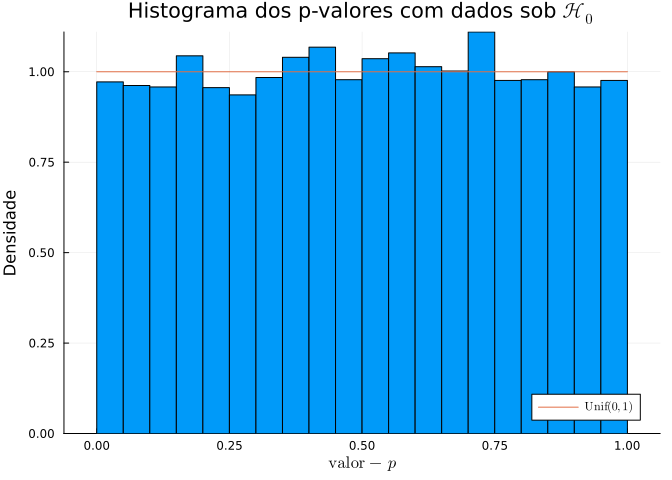
\includegraphics[keepaspectratio]{index_files/mediabag/teste-hipotese_files/figure-pdf/cell-3-output-1.pdf}}

Como é uma função crescente, seu supremo está também no \(0.6\)
Portanto, \[
\begin{aligned}
\alpha_{\max}&=(1-0.6)^2 = 0.16\\
\beta_{\max} &= (1-(1-0.6)^2) = 0.84
\end{aligned}
\]

\section{Teste sob Normalidade}\label{teste-sob-normalidade}

Seja \((x_{n})\) amostra aleatória de \(X\sim N(\mu,\sigma^2)\) em que
\(\sigma^2\) é conhecido. Considere as hipóteses \[
\begin{cases}
H_{0}: \mu = \mu_{0}\\
H_{1}: \mu \neq \mu_{0}
\end{cases}
\] com \(\mu_{0} \in \mathbb{R}\) e fixado.

Calcule as probabilidades (máximas) dos erros tipo I e II, para as
seguintes decisões

\begin{enumerate}
\def\labelenumi{\arabic{enumi}.}
\tightlist
\item
  Se \(\bar{x} < \mu_{0} - 1.96\sqrt{\frac{\sigma^2}{n}}\) ou
  \(\bar{x} > \mu+1.96 \sqrt{ \frac{\sigma^2}{n} }\), então
  \emph{rejeitamos} \(H_{0}\)
\item
  Caso contrário, não rejeitamos \(H_0\)
\end{enumerate}

Temos a função poder \[
\pi(\theta) = P_{\theta}(\mathrm{Rejeitar} H_{0}) = P_{\theta}\left(\bar{X}<\mu_{0} - 1.96 \sqrt{\frac{\sigma^2}{n}}\right)
+P_{\theta}\left( \bar{X} > \mu_{0} + 1.96 \sqrt{  \frac{\sigma^2}{n} } \right)
\]

em que \(theta = \mu \in \mathbb{R}\). Portanto, \[
\alpha_{\max} = \sup_{\theta \in \Theta_{0}} \pi(\theta)
\]

Como \(H_{0}=\mu=\mu_{0} \Leftrightarrow H_{0}: \theta \in \Theta\), em
que \(\Theta_{0}=\{ \mu_{0} \}\), logo,
\(\sup_{\theta \in \Theta_{0}} = \mu_{0}\) Portanto, temos que \[
\alpha_{\max} = \pi(\mu_{0}) = P_{\mu_{0}}\left( \bar{X}<\mu_{0}-1.96\sqrt{ \frac{\sigma^2}{n} } \right) +
P_{\mu_{0}}\left( \bar{X}>\mu_{0} + 1.96 \sqrt{  \frac{\sigma^2}{n} } \right)
\]

Sabemos que, pelo enunciado
\(\bar{X} \sim N\left( \mu, \frac{\sigma^2}{n} \right) \forall \mu \in \mathbb{R}\)
sob \(H_{0}\), ou seja, quando \(\mu= \mu_{0}\) temos que
\(\bar{X}\sim N\left( \mu_{0}, \frac{\sigma^2}{n} \right)\). Note que
\(P_{\mu_{0}}\left( \bar{X}<\mu_{0}-1.96 \sqrt{ \frac{\sigma^2}{n} } \right) =
P_{\mu_{0}}\left(\frac{\bar{X}-\mu_{0}}{\sqrt{ \frac{\sigma^2}{n} }} \right) = 2.5\%\)
Pela simetria da distribuição normal,
\(P_{\mu_{0}}\left( \bar{X}>\mu_{0}+1.96 \sqrt{ \frac{\sigma^2}{n} } \right) = 2.5\%\)
Portanto a probabilidade máxima do erro tipo 1 é \[
\alpha_{\max} = 2.5\% + 2.5\% = 5.0\%
\]

Como
\(H_{1}: \mu \neq \mu_{0} \Leftrightarrow H_{1}: \theta \in \Theta_{1}\),
em que \(\Theta_{1} = \mathbb{R} \setminus \{\mu_{0}\}\), temos que

\[
\begin{aligned}
\beta_{\max} &= \sup_{\theta \in \Theta_{1}}[1-\pi(\theta)] \\
\pi(\theta) &= P_{\theta}\left( \bar{X} < \mu_{0} - 1.96 \sqrt{\frac{\sigma^2}{n}} \right) +
P_{\theta}\left(\bar{X}>\mu_{0}+1.96\sqrt{\frac{\sigma^2}{n}}\right)
\end{aligned}
\]

Sabemos que
\(\bar{X} \sim \mathrm{N}\left( \mu, \frac{\sigma^2}{n} \right)\) para
todo \(\mu \in \mathbb{R}\). Assim, \[
\begin{aligned}
\pi(\theta) &= P_{\theta}\left( \bar{X}<\mu_{0}-1.96 \sqrt{  \frac{\sigma^2}{n} } \right) +
P_{\theta}\left( \bar{X} > \mu_{0} + 1.96 \sqrt{  \frac{\sigma^2}{n} } \right) \\
&= P_{\theta}\left( \frac{\bar{X}-\theta}{\sqrt{ \frac{\sigma^2}{n} }} <
\frac{\mu_{0}-\theta-1.96 \sqrt{  \frac{\sigma^2}{n} } }{\sqrt{  \frac{\sigma^2}{n} }}\right) +
P_{\theta}\left( \frac{\bar{X}-\theta}{\sqrt{ \frac{\sigma^2}{n} }} > 
\frac{\mu_{0}-\theta+1.96 \sqrt{\frac{\sigma^2}{n}}}{\sqrt{\frac{\sigma^2}{n}}}\right)
\end{aligned}
\]

Dessa forma, \[
\beta_{max} = \sup_{\theta \in \Theta_{1}}[1-\pi(\theta)] = 1 - \inf_{\theta \in \Theta_{1}} \pi(\theta)
\]

Ou seja, o supremo dessa expressão é dado por 1 - o ínfimo da função
poder, o que significa que queremos encontrar o valor de \(\theta\) para
o qual
\(P_{\theta}\left( \frac{\bar{X}-\theta}{\sqrt{ \frac{\sigma^2}{n} }} <
\frac{\mu_{0}-\theta-1.96 \sqrt{\frac{\sigma^2}{n} } }{\sqrt{  \frac{\sigma^2}{n} }}\right) +
P_{\theta}\left(\frac{\bar{X}-\theta}{\sqrt{ \frac{\sigma^2}{n} }} >
\frac{\mu_{0}-\theta+1.96 \sqrt{\frac{\sigma^2}{n}}}{\sqrt{\frac{\sigma^2}{n}}}\right)\)
é o menor possível.

Vamos usar \(\mu_0 = 7\) e \(\sigma^2 = 5\) para visualizarmos o
comportamento de \(\alpha\) e \(\beta\)

\pandocbounded{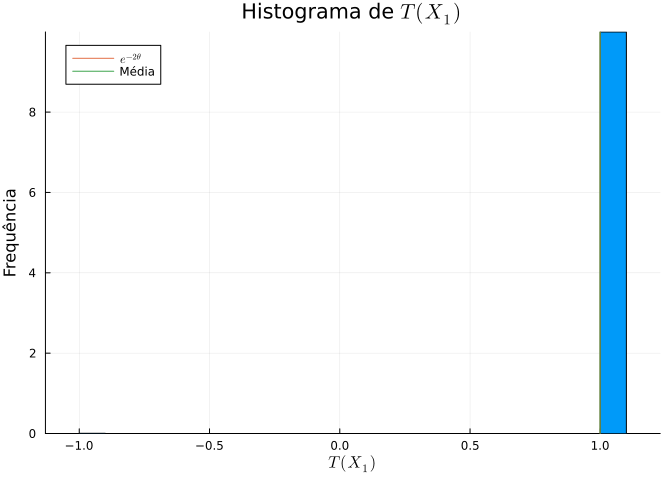
\includegraphics[keepaspectratio]{index_files/mediabag/teste-hipotese_files/figure-pdf/cell-4-output-1.pdf}}

\pandocbounded{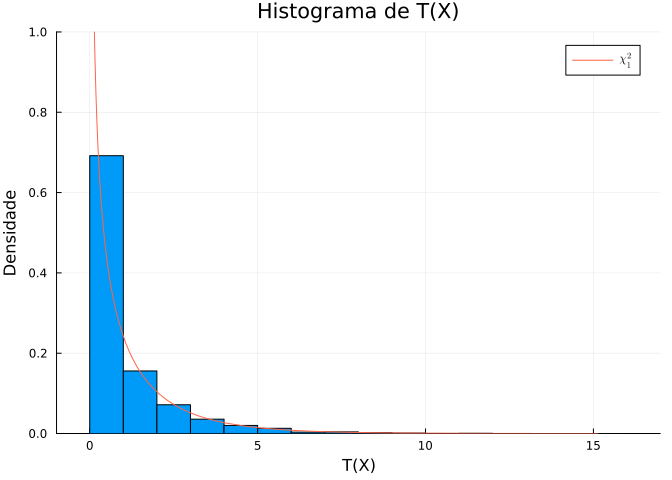
\includegraphics[keepaspectratio]{index_files/mediabag/teste-hipotese_files/figure-pdf/cell-4-output-2.pdf}}

\subsection{Um outro exemplo}\label{um-outro-exemplo}

Seja \((X_{n})\) amostra aleatória de \(X\sim \mathrm{N}(\mu,\sigma^2)\)
com \(\sigma^2 = 5, n = 10\) Com as hipóteses \[
\begin{cases}
H_{0} : \mu = 10 \\
H_{1}: \mu \neq 10
\end{cases}
\] Com as decisões 1. Rejeitamos \(H_{0}\) se
\(\bar{x} > 10 + 1.96 \sqrt{  \frac{5}{10} }\) ou
\(\bar{x} < 10 - 1.96 \sqrt{  \frac{5}{10} }\) Foram observados os
seguintes valores \[
\begin{array}{c}
7.1 & 8.9 & 12 & 13 & 11.7 \\
6.1 & 2.5 & 3.1 & 5.2 & 7
\end{array}
\] Temos então que \(\bar{x} = 7.66\) que, como é abaixo de \(8.6\),
rejeitamos a hipótese nula de que \(\mu = 10\)

\bookmarksetup{startatroot}

\chapter{Procedimento Geral para Testar Hipóteses (Método de
Neyman-Pearson)}\label{procedimento-geral-para-testar-hipuxf3teses-muxe9todo-de-neyman-pearson}

\begin{enumerate}
\def\labelenumi{\arabic{enumi}.}
\tightlist
\item
  Definimos o Modelo Estatístico:

  \begin{enumerate}
  \def\labelenumii{\arabic{enumii}.}
  \tightlist
  \item
    ``Seja \((X_{n})\) amostra aleatória de
    \(x \sim f_{\theta}, \theta \in \Theta\)''
  \end{enumerate}
\item
  Definir as hipóteses de interesse:

  \begin{enumerate}
  \def\labelenumii{\arabic{enumii}.}
  \tightlist
  \item
    \(H_{0}: \theta \in \Theta_{0} \times H_{1}: \theta \in \Theta_{1}\)
    em que
    \(\Theta_{0} \cap \Theta_{1} = \emptyset, \Theta_{0} \neq \emptyset, \Theta_{1}\neq \emptyset, \Theta_{0}\cup \Theta_{1}=\Theta\)
  \end{enumerate}
\item
  A partir da amostra observada, criamos uma regra de decisão para
  verificar a plausibilidade de \(H_{0}\).
\item
  Definimos os pontos de corte da regra de decisão de forma que a
  probabilidade máxima do Erro Tipo I não ultrapasse um limite prefixado
  \(\alpha \in [0,1]\) (normalmente \(5\%\) ou \(1\%\)). Qualquer valor
  \(\geq \alpha\) é dito ser um \emph{nível de significância}.
\item
  Concluímos o Teste de Hipótese.

  \begin{enumerate}
  \def\labelenumii{\arabic{enumii}.}
  \tightlist
  \item
    Se \(H_{0}\) for rejeitado, dizemos que ``Há evidências para
    rejeitar \(H_{0}\) a \(\alpha \cdot [\mathrm{Valor}]\%\) de
    significância estatística''.
  \item
    Se \(H_{0}\) não for rejeitado, dizemos que ``Não há evidências para
    rejeitar \(H_{0}\) a \(\alpha \cdot [\mathrm{Valor}]\%\) de
    significância estatística''
  \item
    Observação: Não rejeitar \(H_{0}\) \emph{não} indica evidência a
    favor de \(H_{0}\), isto é, não sugere que \(H_{0}\) seja
    verdadeiro, apenas que aquela amostra não apresentou evidências
    contrárias.
  \item
    Observação: Quanto menor o valor de \(\alpha\), mais forte será a
    significância estatística.
  \end{enumerate}
\end{enumerate}

\section{Exemplos}\label{exemplos-2}

\subsection{Eexemplo um}\label{eexemplo-um}

Seja \((X_{n})\) a.a de \(X\sim \mathrm{N}(\mu,\sigma^2)\) em que
\(\sigma^2\) é conhecido. Considere (\(\mu_{0}\) fixado)

\[
\begin{cases}
H_{0} : \mu = \mu_{0} \\
H_{1}: \mu \neq \mu_{0}
\end{cases}
\]

\begin{enumerate}
\def\labelenumi{\arabic{enumi}.}
\item
  Construa uma decisão para rejeitar \(H_0\) que produza no máximo
  \(\alpha = 5\%\) (que tenha nível de significância de \(5\%\))

  Como a hipótese alternativa é bilateral, \(H_{1}:\mu\neq \mu_{0}\) e
  \(\bar{x}\) é a EMV para o parâmetro \(\mu\) - a esperança da
  distribuição Normal - definimos a regra: Se \(\bar{x}< x_{a}\) ou
  \(\bar{x}> x_{b}\), rejeitamos \(H_{0}\). Caso contrário, não
  rejeitamos. \[
   \begin{aligned}
       \alpha_{\max} &= \sup_{\theta \in \Theta_{0}} P_{\theta}(\text{Rejeitar }H_{0}), \Theta_{0} = \{ \mu_{0} \} \\
       &= P_{\mu_{0}}(\bar{X}<x_{a}) + P_{\mu_{0}}(\bar{X}>x_{b}) \leq 5\%
   \end{aligned}
   \]

  Note que
  \(\bar{X} \sim \mathrm{N}\left(\mu_{0}, \frac{\sigma^{2}}{n} \right)\),
  sob \(H_{0}\)

  Logo, \[
   \begin{aligned}
       \alpha_{\max} &= P\left( \mathrm{N}(0,1) < \frac{{x_{a}-\mu_{0}}}{\sqrt{ \frac{\sigma^2}{n} }} \right)+
   P\left( \mathrm{N}(0,1) > \frac{{x_{a}-\mu_{0}}}{\sqrt{ \frac{\sigma^2}{n} }} \right)
   \end{aligned}
   \]
\end{enumerate}

::: \{.cell execution\_count=4\} ``` \{.julia .cell-code\} using
Distributions, Plots, StatsPlots, LaTeXStrings

a = plot(Normal(), labels=false) vline!({[}-1.96, 1.96{]}, labels=false)
xticks!({[}-1.96, 1.96{]},
{[}L''\frac{x_{a}-\mu_{0}}{\sqrt{\frac{\sigma^{2}}{n}}}``,
L''\frac{x_{b}-\mu_{0}}{\sqrt{\frac{\sigma^{2}}{n}}}''{]})

display(a) ```

::: \{.cell-output .cell-output-display\}
\pandocbounded{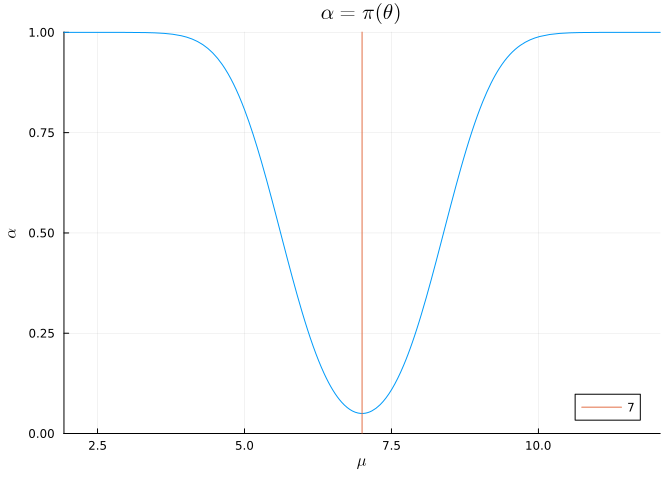
\includegraphics[keepaspectratio]{index_files/mediabag/teste-hipotese_files/figure-pdf/cell-5-output-1.pdf}}
::: :::

\begin{verbatim}
Tomando $\frac{{x_{a}-\mu_{0}}}{\sqrt{\frac{\sigma^2}{n}}} = -1.96$ e $\frac{{x_{b}-\mu_{0}}}{\sqrt{ \frac{\sigma^2}{n}}}
\end{verbatim}

= 1.96\$ (tabela normal padrão simétrica), temos que
\(\alpha_{\max}=5\%\). Assim, resolvendo as equações, \[
    \begin{cases}
       x_{a} = \mu - 1.96 \sqrt{\frac{\sigma^2}{n}} \\
       x_{b} = \mu + 1.96 \sqrt{\frac{\sigma^2}{n}}
    \end{cases}
    \]

\begin{enumerate}
\def\labelenumi{\arabic{enumi}.}
\setcounter{enumi}{1}
\item
  Considere \(n=100\), \(\mu_{0}=1\), \(\sigma^2=0.1\) e
  \(\bar{x}=0.99\). Conclua o teste considerando o mesmo nível de
  significância \(\alpha=5\%\).

  O pontos pontos de corte são \(x_{a} = 0.93\) e \(x_{b} = 1.069\).
  Como \(0.93\leq 0.99 \leq 1.069\), concluímos que não há evidências
  para rejeitarmos \(H_{0}\) a \(5\%\) de significância.
\item
  Refaça considerando \(15\%\) de significância estatística.

  Usando os mesmos argumentos do item 1, podemos encontrar novos valores
  para \(x_{a}, x_{b}\) através da tabela da Normal-Padrão: \[
   \begin{cases}
      x_{a} = \mu - 1.44 \sqrt{\frac{\sigma^2}{n}} \\
      x_{b} = \mu + 1.44 \sqrt{\frac{\sigma^2}{n}}
   \end{cases}
   \]

  Substituindo esses valores para os fornecidos em 2, temos que
  \(0.95 \leq 0.99 \leq 1.045\). Portanto, continuaríamos a dizer que
  não há evidências para rejeitarmos \(H_{0}\) a \(15\%\) de
  significância.
\end{enumerate}

\subsection{2}\label{section}

Seja \((X_{n})\) a.a de \(X\sim \mathrm{N}(\mu,\sigma^2)\) em que
\(\sigma^2\) é conhecido.

Considere (\(\mu_{0}\) fixado)

\[
\begin{cases}
H_{0} : \mu \geq \mu_{0} \\
H_{1}: \mu < \mu_{0}
\end{cases}
\]

\begin{enumerate}
\def\labelenumi{\arabic{enumi}.}
\item
  Construa uma decisão para rejeitar \(H_0\) que produza no máximo
  \(\alpha = 5\%\) (que tenha nível de significância de \(5\%\))

  Pelos parâmetros e hipóteses envolvidos, \((\mu, \text{unilateral})\),
  podemos considerar a seguinte decisão:

  Se \(\bar{x} < x_{c}\), rejeitamos \(H_{0}\). Caso contrário, não
  rejeitamos.

  \[
   \begin{aligned}
       \alpha_{\max} &= \sup_{\mu \geq \mu_{0}} P_{\theta}(\text{Rejeitar }H_{0}) \\
       &= \sup_{\mu\geq \mu_{0}}P_{\mu}(\bar{X}<x_{c}) \\
       \Rightarrow \alpha_{\max} &=\sup_{\mu\geq \mu_{0}}P_{\mu}\left( \mathrm{N}(0,1)< \frac{{x_{c}-\mu}}
   {\sqrt{\frac{\sigma^2}{n} }} \right)
    \end{aligned}
   \]

  Como essa função (acumulada) é decrescente em \(\mu\), temos que \[
   \begin{aligned}
       \alpha_{\max} &= P_{\mu_{0}}(\text{Rejeitar }H_{0}) \\
       &= P_{\mu_{0}}(\bar{X}<x_{c}) \\
       \Rightarrow \alpha_{\max} &=P_{\mu_{0}}\left( \mathrm{N}(0,1)< \frac{{x_{c}-\mu_{0}}}
   {\sqrt{\frac{\sigma^2}{n} }} \right) \leq 5\%
    \end{aligned}
   \]

  Logo, para encontrarmos \(x_{c}\) tal que
  \(\frac{{x_{c}-\mu_{0}}}{\sqrt{ \frac{\sigma^2}{n} }} = -1.64\) (da
  tabela da normal padrão)
  \(\Rightarrow x_{c} = \mu_{0}-1.64 \sqrt{ \frac{\sigma^2}{n} }\)
\item
  Considere \(n=100, \mu_{0} = 1, \sigma^2 = 0.1, \bar{x}=0.99\).
  Conclua o teste anterior a \(\alpha = 5\%\) de significância.

  O ponto de corte é \(x_{c} = 0.9836\). Como \(0.99 \geq 0.9836\),
  concluímos que não há evidências para rejeitar a hipótese nula a
  \(5\%\) de significância.
\end{enumerate}

\subsection{3}\label{section-1}

Seja \((X_{n})\) amostra aleatória de
\(X \sim \mathrm{N}(\mu,\sigma^2)\) em que
\(\theta = (\mu, \sigma^2) = \mathrm{R} \times \mathrm{R}^+\), ou seja,
ambos parâmetros são desconhecidos.

\[
\begin{cases}
H_{0} : \sigma^2 = \sigma^2_{0} \\
H_{1}: \sigma^2 \neq \sigma^2_{0}
\end{cases} \Rightarrow 
\begin{aligned}
& \text{Decisão com significância } \alpha \\
&\text{Rejeita $H_{0}$ se} \\
&\begin{cases}
s^2 < c_{1c} \\
s^2 > c_{2c} \\
\end{cases} \\
& \text{Em que $c_{1c},c_{2c}$ são tais que} \\
& \sup_{\theta\in\Theta_{0}}P_{\theta}(\text{Erro Tipo I}) = \alpha_{\max} = \alpha \\
&\text{E } s^2 = \frac{1}{n-1} \sum^n_{i=1}(x_{i}-\bar{x})^2
\end{aligned} \\ \\
\]

Sabemos que
\(\frac{\sum_{i=1}^n(X_{i}-\bar{X})^2}{\sigma^2}\sim \chi^2_{n-1},\forall \mu \in \mathbb{R}, \sigma^2 > 0\).
Em particular, sob \(H_{0}\) \[
\begin{aligned}
&\frac{(n-1)s^2(\underset{\sim}{X_{n}})}{\sigma^2_{0}} \sim \chi^2_{n-1}
\\ \Rightarrow& \alpha_{\max} = \sup_{\theta \in \Theta_{0}}\left\{ P_{\theta}(s^2(\underset{\sim}{X_{n}}) < c_{1c}) +
P_{\theta}(s^2(\underset{\sim}{X_{n}})> c_{2c}) \right\} 
\end{aligned}
\]

Além disso, note que
\(\Theta_{0}=\{ (\mu,\sigma^2)\in \Theta:\sigma^2=\sigma^2_{0} \}\).
Portanto, temos que \[
\begin{aligned}
& \alpha_{\max} = \sup_{\theta \in \Theta_{0}} \underbracket{ \left\{  P\left( \chi^2_{n-1} < 
\frac{c_{1c}(n-1)}{\sigma^2_{0}}\right) + P\left( \chi^2_{n-1} > 
\frac{c_{2c}(n-1)}{\sigma^2_{0}} \right) \right\}}_{\text{Não depende de $\theta$}}\\
\Rightarrow & \alpha_{\max} =  P\left( \chi^2_{n-1} < \frac{c_{1c}(n-1)}{\sigma^2_{0}} \right) + P\left( \chi^2_{n-1} >
\frac{c_{2c}(n-1)}{\sigma^2_{0}} \right) 
\end{aligned}
\]

Fixando \(\alpha_{\max}=\alpha\) (significância), encontramos pela
tabela os valores de
\(q_{\frac{\alpha}{2},n-1}^{(1)}, q_{\frac{\alpha}{2},n-1}^{(2)}\) tais
que dividam a distribuição \(\chi^2_{n-1}\) criando duas seções de
\(\frac{\alpha}{2}\) de área. Portanto,

\[
\begin{cases}
H_{0} : \sigma^2 = \sigma^2_{0} \\
H_{1}: \sigma^2 \neq \sigma^2_{0}
\end{cases} \Rightarrow 
\begin{aligned}
& \text{Decisão com significância } \alpha \\
&\text{Rejeita $H_{0}$ se} \\
&\begin{cases}
s^2 < q_{\frac{\alpha}{2},n-1}^{(1)} \cdot \frac{\sigma^2_{0}}{(n-1)} \\
s^2 > q_{\frac{\alpha}{2},n-1}^{(2)} \cdot \frac{\sigma^2_{0}}{(n-1)}\\
\end{cases}
\end{aligned}
\]

\subsection{Exemplo}\label{exemplo-7}

Seja \((X_{n})\) amostra aleatória de \(X\sim N(\mu,\sigma^2)\) em que
\(X\) é o peso do pacote de café. Colheu-se uma amostra de \(n=16\)
pacotes e observou-se uma variância de \(s^2 =169g^2\). O processo de
fabricação diz que a média dos pacotes é \(500g\) e desvio-padrão 10
gramas (\(\sigma^2_{0}=100g^2\)).

Queremos verificar se há alguma evidência de que o processo não esteja
sendo cumprido com \(\alpha=5\%\) de significância \[
\begin{cases}
H_{0} : \sigma^2 = 100 \\
H_{1}: \sigma^2 \neq 100
\end{cases} \Rightarrow 
\begin{aligned}
& \text{Decisão com significância } 5\% \\
&\text{Rejeita $H_{0}$ se} \\
&\begin{cases}
s^2 < q_{2.5\%,15}^{(1)} \cdot \frac{100}{15} \\
s^2 > q_{2.5\%,15}^{(2)} \cdot \frac{100}{15}\
\end{cases}
\end{aligned}
\] Da tabela Qui-quadrado, temos \(q_{2.5\%,15}^{(1)} = 6.26\) e
\(q_{2.5\%,15}^{(2)} =27.49\).

Como \(41.73<100<183.26\), concluímos que não há evidências para
rejeitar a hipótese nula a \(5\%\) de significância

\bookmarksetup{startatroot}

\chapter{Fórmulas}\label{fuxf3rmulas}

\section{Sob normalidade, variância
conhecida}\label{sob-normalidade-variuxe2ncia-conhecida}

Seja \((X_{n})\) amostra aleatória de \(X\sim \mathrm{N}(\mu,\sigma^2)\)
em que \(\sigma^2\) é conhecido. \[
\begin{aligned}
&1.
\begin{cases}
H_{0} : \mu = \mu_{0} \\
H_{1}: \mu \neq \mu_{0}
\end{cases} \Rightarrow 
\begin{aligned}
& \text{Decisão com significância } \alpha \\
&\text{Rejeita $H_{0}$ se} \\
&\begin{cases}
\bar{x} < \mu_{0} - z_{\frac{\alpha}{2}} \sqrt{ \frac{\sigma^2}{n} } \\
\bar{x} > \mu_{0} + z_{\frac{\alpha}{2}} \sqrt{ \frac{\sigma^2}{n} }
\end{cases} \\
& \text{Em que $z_{\frac{\alpha}{2}}$ é tal que} \\
& P\left( \mathrm{N(0,1)} < z_{\frac{\alpha}{2}} \right) = \frac{\alpha}{2}
\end{aligned} \\ \\
& 2.
\begin{cases}
H_{0} : \mu \geq \mu_{0} \\
H_{1}: \mu < \mu_{0}
\end{cases} \Rightarrow 
\begin{aligned}
&\text{Rejeita $H_{0}$ se} \\
&\begin{cases}
\bar{x} < \mu_{0} - z_{\alpha} \sqrt{ \frac{\sigma^2}{n} } \\
\end{cases} \\
& \text{Em que $z_{\alpha}$ é tal que} \\
& P\left( \mathrm{N(0,1)} \leq z_{\alpha} \right) = \alpha
\end{aligned} \\ \\
& 3.
\begin{cases}
H_{0} : \mu \leq \mu_{0} \\
H_{1}: \mu > \mu_{0}
\end{cases} \Rightarrow 
\begin{aligned}
&\text{Rejeita $H_{0}$ se} \\
&\begin{cases}
\bar{x} > \mu_{0} + z_{\alpha} \sqrt{ \frac{\sigma^2}{n} } \\
\end{cases} \\
& \text{Em que $z_{\alpha}$ é tal que} \\
& P\left( \mathrm{N(0,1)} \geq z_{\alpha} \right) = \alpha
\end{aligned} \\
\end{aligned}
\]

\section{Sob normalidade, variância
desconhecida}\label{sec-normalidade-vardesc}

Seja \((X_{n})\) amostra aleatória de
\(X \sim \mathrm{N}(\mu,\sigma^2)\) em que
\(\theta = (\mu, \sigma^2) = \mathrm{R}
\times \mathrm{R}^+\), ou seja, ambos parâmetros são desconhecidos. \[
\begin{aligned}
&1.
\begin{cases}
H_{0} : \mu = \mu_{0}  \\
H_{1} : \mu \neq \mu_{0} \\
\Rightarrow \Theta_{0}=\{ (\mu,\sigma^2) \in \Theta : \mu = \mu_{0} \}\\
\Rightarrow \Theta_{1}=\{ (\mu,\sigma^2) \in \Theta : \mu \neq \mu_{0} \}\\ 
\end{cases} \Rightarrow 
\begin{aligned}
& \text{Decisão com significância } \alpha \\
&\text{Rejeita $H_{0}$ se} \\
&\begin{cases}
\frac{\bar{x}-\mu_{0}}{\sqrt{ \frac{s^2}{n} }} < - t_{\frac{\alpha}{2},n-1} \\
\frac{\bar{x}-\mu_{0}}{\sqrt{ \frac{s^2}{n} }} > t_{\frac{\alpha}{2},n-1} \\
\end{cases} \\
& \text{Em que $t_{\frac{\alpha}{2},n-1}$ é tal que} \\
& P\left( t_{n-1} < - t_{\frac{\alpha}{2},n-1} \right) = \frac{\alpha}{2}
\end{aligned} \\ \\
& 2.
\begin{cases}
H_{0} : \mu \geq \mu_{0} \\
H_{1}: \mu < \mu_{0}
\end{cases} \Rightarrow 
\begin{aligned}
&\text{Rejeita $H_{0}$ se} \\
&\begin{cases}
\frac{\bar{x}-\mu_{0}}{\sqrt{ \frac{s^2}{n} }} < - t_{\alpha,n-1} \\
\end{cases} \\
& \text{Em que $t_{\alpha,n-1}$ é tal que} \\
& P\left( t_{n-1}\leq -t_{\alpha,n-1} \right) = \alpha
\end{aligned} \\ \\
& 3.
\begin{cases}
H_{0} : \mu \leq \mu_{0} \\
H_{1}: \mu > \mu_{0}
\end{cases} \Rightarrow 
\begin{aligned}
&\text{Rejeita $H_{0}$ se} \\
&\begin{cases}
\frac{\bar{x}-\mu_{0}}{\sqrt{ \frac{s^2}{n} }} > - t_{\alpha,n-1} \\
\end{cases} \\
& \text{Em que $t_{\alpha,n-1}$ é tal que} \\
& P\left( t_{n-1} > t_{\alpha,n-1} \right) = \alpha
\end{aligned} \\
\end{aligned}
\]

Em que \(s^2 = \frac{1}{n-1} \sum^n_{i=1}(x_{i}-\bar{x})^2\) é a
variância amostral (não enviesada)

\section{Sob normalidade, para a
variância.}\label{sob-normalidade-para-a-variuxe2ncia.}

Seja \((X_{n})\) amostra aleatória de
\(X \sim \mathrm{N}(\mu,\sigma^2)\) em que
\(\theta = (\mu, \sigma^2) = \mathrm{R} \times \mathrm{R}^+\), ou seja,
ambos parâmetros são desconhecidos. \[
\begin{cases}
H_{0} : \sigma^2 = \sigma^2_{0} \\
H_{1}: \sigma^2 \neq \sigma^2_{0}
\end{cases} \Rightarrow 
\begin{aligned}
& \text{Decisão com significância } \alpha \\
&\text{Rejeita $H_{0}$ se} \\
&\begin{cases}
s^2 < q_{\frac{\alpha}{2},n-1}^{(1)} \cdot \frac{\sigma^2_{0}}{(n-1)} \\
s^2 > q_{\frac{\alpha}{2},n-1}^{(2)} \cdot \frac{\sigma^2_{0}}{(n-1)}\\
\end{cases}
\end{aligned}
\]

Em que \(s^2 = \frac{1}{n-1} \sum^n_{i=1}(x_{i}-\bar{x})^2\) é a
variância amostral (não enviesada) e
\(q_{\frac{\alpha}{2},n-1}^{(1)}, q_{\frac{\alpha}{2},n-1}^{(2)}\) tais
que dividam a distribuição \(\chi^2_{n-1}\) criando duas seções de
\(\frac{\alpha}{2}\) de área.

\bookmarksetup{startatroot}

\chapter{Teste de Hipótese para duas
populações}\label{teste-de-hipuxf3tese-para-duas-populauxe7uxf5es}

Sejam \(X, Y\) duas variáveis de interesse representando duas
sub-populações. Estamos interessados em verificar se a média
populacional de \(X\) é menor, maior ou igual à de \(Y\). Sendo assim,
precisamos considerar os casos em que \(X\) é independente de \(Y\) e o
caso em que não são independentes (pareados).

\section{Dados independentes e
dependentes}\label{dados-independentes-e-dependentes}

Um pesquisador propôs um novo método de investimento para aumentar o
rendimento mensal. Selecionou 20 investidores aleatoriamente de um
universo de investidores cadastrados. Em um primeiro momento, o
pesquisador deixou os investidores investirem do jeito que sabem e ao
final verificou a renda obtida. \(X\) é o rendimento dos investidores
sem ter o conhecimento do método.

Então, o pesquisador ensinou seu método aos investidores, onde \(Y\)
passou a ser o rendimento dos investidores após a aplicação do método
ensinado.

Claramente, \(X,Y\) são dependentes.

O mesmo pesquisador testará o mesmo método de forma diferente. Para
testar o seu método, o pesquisador selecionou 20 indivíduos com
características similares do universo de investidores, dos quais

\begin{enumerate}
\def\labelenumi{\arabic{enumi}.}
\item
  10 foram designados aleatoriamente a não receber o método \(X:\)
  rendimento de um indivíduo que não recebeu o método
\item
  10 foram designados aleatoriamente a receberem o método \(Y:\)
  rendimento de um indivíduo que recebeu o método
\end{enumerate}

Nesse caso, as variáveis \(X,Y\) são independentes.

Em ambas abordagens, temos as mesmas hipóteses de interesse: \[
1.
\begin{cases}
H_{0}:\mu_{X}\geq \mu_{y} \\
H_{1}: \mu_{X} < \mu_{Y}
\end{cases} ~~~2.
\begin{cases}
H_{0}:\mu_{X}\leq \mu_{Y} \\
H_{1}: \mu_{X} > \mu_{Y}
\end{cases} ~~~3.
\begin{cases}
H_{0}:\mu_{X}= \mu_{Y} \\
H_{1}: \mu_{X} \neq \mu_{Y}
\end{cases}
\]

Podemos definir \(\mu_{D}=\mu_{X}-\mu_{Y}\) e reescrever as hipóteses \[
1.
\begin{cases}
H_{0}:\mu_{D} \geq 0 \\
H_{1}: \mu_{D} < 0
\end{cases} ~~~2.
\begin{cases}
H_{0}:\mu_{D} \leq 0 \\
H_{1}: \mu_{D} > 0
\end{cases} ~~~3.
\begin{cases}
H_{0}:\mu_{D} = 0 \\
H_{1}: \mu_{D} \neq 0
\end{cases}
\]

Para os próximos exemplos, assumiremos normalidade para \(X,Y\)

\subsection{Caso pareado (variáveis
dependentes)}\label{caso-pareado-variuxe1veis-dependentes}

No caso em que \(X,Y\) são dependentes, as amostras são \((X_{n})\)
\hyperref[sec-aa]{amostras aleatórias} de \(X\) e \((Y_{n})\) a.a de
\(Y\) tais que \(X_{i},Y_{i}\) são dependentes.

Para este caso, fazemos \(D_{i}=X_{i}-Y_{i},i=1,2,\dots, n\). Temos que
\((D_{n})\) é uma amostra aleatória de
\(D=X-Y \sim N(\mu_{D},\sigma^2_{D})=N(\mu_{X}-\mu_{Y},\sigma^2_{X}+\sigma^2_{Y}-2 \rho\sigma_{X}\sigma _{Y})\)

Observe ainda que \[
\bar{D}_{\mathrm{Par}}=\sum^{n}_{i=1} \frac{D_{i}}{n} \sim N\left( \mu_{D}, \frac{\sigma^2_{D}}{n} \right)
\] Note ainda que as variância e covariância de \(X,Y\) estão embutidas
em \(\sigma^2_{D}\). Podemos usar \[
s^2_{D}(\underset{\sim}{D})=\frac{1}{n-1}\sum^n_{i=1}(D_{i}-\bar{D}_{\mathrm{Par}})^2
\] Para estimar \(\sigma^2_{D}\) Podemos construir as decisões como já
vimos anteriormente em \hyperref[sec-normalidade-vardesc]{testes sob
normalidade com variância desconhecida}.

\subsection{Exemplo}\label{exemplo-8}

Foram coletados os rendimentos (em mil reais) antes e após a aplicação o
método para 12 investidores. Queremos verificar se o método aumentou o
rendimento médio. Chamaremos de \(X\) o rendimento anterior ao
treinamento e \(Y\) o rendimento após. Isto é, queremos verificar se
\(\mu_{D}=\mu_{X}-\mu_{Y}\leq 0\). Portanto, nossa hipótese nula é de
que o treinamento não tem efeito positivo no rendimento:

\[
\begin{cases}
H_{0}:\mu_{D} \geq 0 \\
H_{1}: \mu_{D} < 0
\end{cases}
\]

\[
\begin{array}{c|c|c|c}
\mathrm{Indíce}  & \mathrm{Antes}(X)  &  \mathrm{Depois}(Y) & \mathrm{Dif}(D) & \mathrm{Dif^2}(D^2)\\
\hline
1 & 2.4 &  4.3 & -1.9 & 3.61\\
2 & 2.8  & 3.4  & -0.6 & 0.36\\
3 & 4.6  & 3.2  & 1.4 & 1.96\\
4 & 3.1  & 3.3 & -0.2 & 0.04\\
5 & 3.1  & 3.3 & -0.2 & 0,04\\
6 & 4.7 &  5.8 & -1.1 & 1.21\\
7 & 3.5  & 3.8 & -0.3 & 0.09\\
8 & 1.7  & 3.5 & -1.8 & 3.24\\
9 & 2.3  & 3.2 & -0.9 & 0.81\\
10 & 2.6  & 3.9 & -1.3 & 1.69\\
11 & 4.2  & 3.6 & 0.6 & 0.36\\
12 & 3.4  & 4.3  & -0.9  & 0.81\\
\hline
\mathrm{Média}  & 3.2  & 3.8  & -0.6 \\
s^2 & 0.87  & 0.55  &  0.9
\end{array}
\]

Temos que \(s^2(\underset{\sim}{D})=0.9\). (Podemos calcular diretamente
ou usando a coluna \(D^2\) e substituindo no somatório
\(s^2_{D}=\left( \frac{\sum^n_{i=1}d_{i}^2}{n}-\bar{d}^2 \right) \frac{n}{n-1}\)
) Rejeitamos \(H_{0}\) se
\(\frac{\bar{d}_{\mathrm{Par}}}{\sqrt{ \frac{s^2_{D}}{n}}}<-t_{\alpha,n-1}\)
onde \(t_{\alpha,n-1}\) é tal que \(P(t_{n-1}<-t_{\alpha,n-1})=\alpha\),
onde \(t_{n-1}\) é a distribuição T de Student com \(n-1\) graus de
liberdade.

Temos que
\(\frac{\bar{d}_{\mathrm{Par}}}{\sqrt{ \frac{s^2_{D}}{n}}} =-2.19\) e, a
\(\alpha=0.05\), \(-t_{0.05,11}=-1.796\). Como \(-2.19< -1.796\),
podemos dizer que há evidências de que o método aumenta o rendimento
médio dos investidores a \(5\%\) de significância. Por outro lado, com
\(\alpha=0.01, -t_{0.01,11}=-2.718\) e, por \(-2.19\geq -2.718\),
dizemos que não há evidências para rejeitar a hipótese de que o método
não aumenta o rendimento (rejeitar a hipótese nula) a 1\% de
significância estatística.

\section{Caso de independência}\label{caso-de-independuxeancia}

Sejam \(X, Y\) variáveis aleatórias \emph{independentes} tais que
\[ \begin{cases}
X\sim N(\mu_{X},\sigma^2_{X}) \\
Y\sim (\mu_{Y},\sigma^2_{Y})
\end{cases} \] Considere \((X_{n})\) amostra aleatória de \(X\) e
\((Y_{m})\). Estamos interessados em testar as hipóteses: \[
1.
\begin{cases}
H_{0}:\mu_{X}\geq \mu_{Y} \\
H_{1}: \mu_{X} < \mu_{Y}
\end{cases} ~~~2.
\begin{cases}
H_{0}:\mu_{X}\leq \mu_{Y} \\
H_{1}: \mu_{X} > \mu_{Y}
\end{cases} ~~~3.
\begin{cases}
H_{0}:\mu_{X}= \mu_{Y} \\
H_{1}: \mu_{X} \neq \mu_{Y}
\end{cases}
\] Podemos definir \(\mu_{D}=\mu_{X}-\mu_{Y}\) e obter a equivalência
dessas hipóteses \[
1.
\begin{cases}
H_{0}:\mu_{D} \geq 0 \\
H_{1}: \mu_{D} < 0
\end{cases} ~~~2.
\begin{cases}
H_{0}:\mu_{D} \leq 0 \\
H_{1}: \mu_{D} > 0
\end{cases} ~~~3.
\begin{cases}
H_{0}:\mu_{D} = 0 \\
H_{1}: \mu_{D} \neq 0
\end{cases}
\] Considere \[
\bar{D}_{\mathrm{NPar}}=\bar{X}-\bar{Y}
\]

Como
\(\bar{X}\sim N\left( \mu_{X}, \frac{\sigma^2_{X}}{n} \right), \bar{Y} \sim N\left( \mu_{Y}, \frac{\sigma^2_{Y}}{m} \right)\),
temos que
\(\bar{D}_{\mathrm{NPar}} \sim N\left( \mu_{D}, \frac{\sigma^2_{X}}{n} + \frac{\sigma^2_{Y}}{m} \right)\)

\subsection{Ambas variâncias
conhecidas}\label{ambas-variuxe2ncias-conhecidas}

Podemos substituir o valor numérico das variâncias na distribuição de
\(\bar{D}_{\mathrm{NPar}}\), obtendo uma distribuição normal com pontos
de corte para as decisões:

\[
\begin{aligned}
1. &\text{ Rejeita $H_{0}$ se } \bar{d}_{\mathrm{NPar}} < -z_{\alpha} \underbrace{\sqrt{ \frac{\sigma^2}{n} +
\frac{\sigma^2}{m} }}_{\mathrm{Var}(\bar{D}_{\mathrm{NPar}})}, \sigma_{2}=\sigma^2_{X}=\sigma^2_{Y} \\
2. & \text{ Rejeita $H_{0}$ se } \bar{d}_{\mathrm{NPar}} > z_{\alpha} \sqrt{ \frac{\sigma^2}{n} + \frac{\sigma^2}{m} } \\
3. & \text{ Rejeita $H_{0}$ se } \bar{d}_{\mathrm{NPar}} < -z_{\frac{\alpha}{2}} \sqrt{ \frac{\sigma^2}{n} +
\frac{\sigma^2}{m} } \text{ ou } \bar{d}_{NPar} > z_{\alpha} \sqrt{ \frac{\sigma^2}{n} + \frac{\sigma^2}{m} }
\end{aligned}
\]

\subsection{Variâncias desconhecidas e
iguais}\label{variuxe2ncias-desconhecidas-e-iguais}

Temos que \(\sigma^2_{X}=\sigma^2_{Y}=\sigma^2\) é conhecido.

\subsubsection{Estimando via t-Student}\label{estimando-via-t-student}

Através da distribuição t-Student com \(n+m-2\) graus de liberdade,
podemos estimar os pontos de corte. Temos nossas decisões: \[
\begin{aligned}
1. &\text{ Rejeita $H_{0}$ se } \bar{d}_{\mathrm{NPar}} < -t_{n+m-2,\alpha} \sqrt{ \frac{s_{p}^2}{n} + \frac{s_{p}^2}{m} } \\
2. & \text{ Rejeita $H_{0}$ se } \bar{d}_{\mathrm{NPar}} > t_{n+m-2,\alpha} \sqrt{ \frac{s^2_{p}}{n} + \frac{s^2_{p}}{m} } \\
3. & \text{ Rejeita $H_{0}$ se } \bar{d}_{\mathrm{NPar}} < -t_{n+m-2,\frac{\alpha}{2}} \sqrt{ \frac{s^2_{p}}{n} +
\frac{s^2_{p}}{m} } \text{ ou } \bar{d}_{NPar} > t_{n+m-2, \frac{\alpha}{2}} \sqrt{ \frac{s^2_{p}}{n} + \frac{s^2_{p}}{m} }
\end{aligned}
\] Onde \(s^2_{p}= \frac{(n-1)s^2_{X}+(m-1)s^2_{Y}}{n+m-2}\), com
\(s^2_{X}, s^2_{Y}\) sendo os estimadores não enviesados para as
variâncias de \(X\) e \(Y\), respectivamente. (Ponderamos os estimadores
com base no tamanho de sua amostra, assim favorecendo os estimadores
mais precisos)

\subsection{Variâncias desconhecidas e diferentes (caso
geral)}\label{variuxe2ncias-desconhecidas-e-diferentes-caso-geral}

Temos que \(\sigma^2_{X},\sigma^2_{Y}\) são desconhecidos e diferentes.

\subsubsection{Estimando via t-Student}\label{estimando-via-t-student-1}

usaremos a distribuição t-Student com \(n'\) graus de liberdade. Temos
nossas decisões:

\[
\begin{aligned}
1. &\text{ Rejeita $H_{0}$ se } \bar{d}_{\mathrm{NPar}} < -t_{n',\alpha} \sqrt{ \frac{s_{p}^2}{n} + \frac{s_{p}^2}{m} } \\
2. & \text{ Rejeita $H_{0}$ se } \bar{d}_{\mathrm{NPar}} > t_{n',\alpha} \sqrt{ \frac{s^2_{p}}{n} + \frac{s^2_{p}}{m} } \\
3. & \text{ Rejeita $H_{0}$ se } \bar{d}_{\mathrm{NPar}} < -t_{n',\frac{\alpha}{2}} \sqrt{\frac{s^2_{p}}{n} + \frac{s^2_{p}}{m}}
\text{ ou } \bar{d}_{NPar} > t_{n', \frac{\alpha}{2}} \sqrt{ \frac{s^2_{p}}{n} + \frac{s^2_{p}}{m} }
\end{aligned}
\]

Onde \(s^2_{p}= \frac{(n-1)s^2_{X}+(m-1)s^2_{Y}}{n+m-2}\).

\paragraph{\texorpdfstring{Encontrando
\(n’\)}{Encontrando n'}}\label{encontrando-n}

Na fórmula acima, temos os graus de liberdade da t-Student dado por \[
n' \approx \frac{\left(\frac{s^2_{X}}{n}+\frac{s^2_{Y}}{m}\right)^2}{\frac{\left(\frac{s^2_{X}}{n}\right)^2}
{n-1}+\frac{\left(\frac{s^2_{Y}}{m}\right)^2}{m-1}}
\] Esse valor, caso não inteiro, deverá ser arredondado.

\subsubsection{Exemplo (Importante)}\label{exemplo-importante}

Queremos testar a resistência de dois tipos de viga de aço, \(A\) e
\(B\). Tomando-se \(n=15\) vigas do tipo \(A\) e \(m=20\) vigas do tipo
\(B\). de um teste \(f\), conseguimos com \(10\%\) de significância que
as variâncias não são iguais. Obtemos os valores da tabela: \[
\begin{array}{c|c}
\text{Tipo}  & \text{Média}  & \text{Variância} (s^2) \\
\hline
A & 70.5 & 81.6 \\
B  & 84.3  & 210.8 \\
\bar{d}_{\mathrm{NPar}}  & -13.8 & --
\end{array}
\] Teste a hipótese \[
\begin{cases}
H_{0} : \mu_{X} = \mu_{Y} \\
H_{1}:\mu_{X} \neq \mu_{Y}
\end{cases}
\] Com significância \(\alpha = 0.05\) para os casos \#\#\#\#\# Caso 1.
Variâncias conhecidas Temos do produtor que
\(\sigma^2_{X}=81, \sigma^2_{Y}=209\)
\(\bar{d}_{\mathrm{NPar}}=70.5-84.3 = -13.8\). Logo,
\(z_{\frac{\alpha}{2}}\sqrt{ \frac{81}{15} + \frac{209}{20}}=7.8\). Como
\(-13.8 < -7.8\), concluímos que há evidências para rejeitarmos a
hipótese nula de que as resistências médias das vigas \(A,B\) são iguais
a \(\alpha = 5\%\) de significância estatística

\paragraph{Caso 2. Variâncias desconhecidas e
iguais.}\label{caso-2.-variuxe2ncias-desconhecidas-e-iguais.}

Para \(\alpha=0.05\), \(t_{33,0.025}=2.03\). Encontrando
\(s^2_{P} = 155.988\). Finalmente, \(t_{33,0.025}
\sqrt{  \frac{s^2_{P}}{n} + \frac{s^2_{P}}{m} }=8.65\). Como
\(-13.8 < -8.65\), concluímos que há evidências para rejeitarmos a
hipótese nula a \(\alpha=5\%\) de significância estatística.

\paragraph{Caso 3. Variâncias desconhecidas e
diferentes}\label{caso-3.-variuxe2ncias-desconhecidas-e-diferentes}

Primeiro calculamos \(n'= 32.08 \stackrel{\text{Arrendonda}}{=}32\).
Assim, \(t_{32,0.025} = 2.037\). Portanto,
\(t_{32,0.025} \sqrt{  \frac{s^2_{X}}{n} + \frac{s^2_{Y}}{m} }=8.14\).
Como \(-13.8 < -8.15\), concluímos que há evidências para rejeitarmos a
hipótese nula a \(\alpha=5\%\) de significância estatística.

\bookmarksetup{startatroot}

\chapter{Tabela de frequências}\label{tabela-de-frequuxeancias}

Sejam \(X,Y\) variáveis aleatórias cujos valores observados são
\(B_{1},B_{2},\dots,B_{l}\) e \(A_{1},A_{2}, A_{k}\), respectivamente.
Observam-se os seguintes dados \[
\begin{array}{ccc}
\mathrm{ind.}  & X & Y \\
1  & B_{2} & A_{1} \\
2 & B_{7} & A_{3} \\
\vdots & \vdots  & \vdots \\
n  & B_{1} & A_{5}
\end{array}
\] Colocamos nossos dados numa tabela de frequências absolutas
observadas \[
\begin{array}{c|cccc|c}
X\setminus Y  & A_{1} & A_{2} & \dots & A_{k} & \mathrm{Total}~X \\
\hline
B_{1} & O_{11} & O_{12} & \dots & O_{1k} & O_{1\cdot} \\
B_{2} & O_{11} & O_{12} & \dots & O_{1k} & O_{2\cdot} \\
\vdots & \vdots & \vdots & \ddots & \vdots & \vdots \\
B_{l} & O_{l1} & O_{l2} & \dots & O_{lk} & O_{l\cdot} \\
\hline
\mathrm{Total}~Y  & O_{\cdot_{1}} & O_{\cdot_{2}}  & \dots  & O_{\cdot k}  & n
\end{array}
\]

Temos nossa tabela de frequências esperadas {[}{[}Teste de
Hipótese\textbar sob{]}{]} \(H_{0}\) (Independência) \[
\begin{array}{c|cccc|c}
X\setminus Y  & A_{1} & A_{2} & \dots & A_{k} & \mathrm{Total}~X \\
\hline
B_{1} & E_{11} & E_{12} & \dots & E_{1k} & O_{1\cdot} \\
B_{2} & E_{11} & E_{12} & \dots & E_{1k} & O_{2\cdot} \\
\vdots & \vdots & \vdots & \ddots & \vdots & \vdots \\
B_{l} & E_{l1} & E_{l2} & \dots & E_{lk} & O_{l\cdot} \\
\hline
\mathrm{Total}~Y  & O_{\cdot_{1}} & O_{\cdot_{2}}  & \dots  & O_{\cdot k}  & n
\end{array}
\] Em que \[
E_{ij} = \frac{O_{i \cdot} \cdot O_{\cdot j}}{n}
\] Note que, sob independência \[
\begin{aligned}
P(B_{i}\cap A_{j}) &= P(B_{i}) \cdot P(A_{j}) \\
E_{ij} &= n \cdot P(B_{i}\cap A_{j}) \stackrel{\mathrm{ind.}}{=} n P(B_{i}) \cdot P_{A_{j}}
\end{aligned}
\] Estimando \(P(B_{i}), P(A_{j})\) temos \[
\widehat{P(B_{i})} = \frac{O_{i\cdot}}{n}, \widehat{P(A_{j})}= \frac{O_{\cdot j}}{n}
\] Logo, o valor esperado estimado é \[
\widehat{E_{ij}}=n \cdot \widehat{P(B_{i})}\cdot\widehat{P(A_{j})} = \frac{O_{i \cdot} \cdot O_{\cdot j}}{n}
\]

Em ambos testes, usaremos a seguinte estatística para testar suas
hipóteses (independência e homogeneidade) \[
\chi^2 = \sum^k_{i=1}\sum^l_{j=1} \frac{(O_{ij}-E_{ij})^2}{E_{ij}}
\] Sob \(H_{0}\), ou seja, \[
\chi^2_{obs}\sim \chi^2_{(k-1)(l-1)}
\] Dessa forma, rejeitamos a hipótese \(H_{0}\) a \(\alpha\) graus de
liberdade se \[
\chi^2_{obs} > c_{p}
\] em que \(c_{p}\) satisfaz \(P(\chi^2_{(k-1)(l-1)} > c_{p})=\alpha\).

\emph{Observação} Essa aproximação com a \(\chi^2\) só funciona de modo
razoável quando cada \(E_{ij}>5\)

\bookmarksetup{startatroot}

\chapter{Teste Qui-Quadrado e análise de
aderência}\label{teste-qui-quadrado-e-anuxe1lise-de-aderuxeancia}

A análise de aderência \href{teste-hipotese.qmd}{testa} a distribuição
dos dados: \[
\begin{cases}
H_{0}: P= P_{0} \\
H_{1}: P \neq P_{0}
\end{cases}
\] Em que \(P_{0}\) é a medida de probabilidade especificada que
governaria (sob \(H_0\)) os eventos observados.

Neste teste co,paramos a frequência observada com a frequência esperada
em \(k\) eventos disjuntos e distintos observáveis. \[
\begin{array}{c|cc}
\text{Eventos}  & 1  & 2 & \dots & k \\
\hline
P_{0} & P_{01} & P_{02} & \dots & P_{0k} \\
E_{i}  & E_{1} & E_{2} & \dots & E_{k} \\
O_{i} & O_{1} & O_{2} & \dots & O_{k}
\end{array}
\]

Em que observou-se uma \hyperref[sec-ao]{amostra} de tamanho \(n\).
Temos também que \(E_{i}\) é o valor esperado do número de eventos \(i\)
sob \(H_{0}\) \[
\mathrm{Freq. Esperada} = E_{i} = P_{0i} \cdot n
\]

e \(\mathrm{Freq. Observada} = O_{i}\) é o numero real de eventos \(i\)
observados na amostra. A \href{estatisticas.qmd}{estatística} para
testar \(H_{0}\) é \[
\chi^2 = \sum^k_{i=1} \frac{(E_{i}-O_{i})^2}{E_{i}}
\]

que, sob \(H_0\) - ou seja, sob a hipótese de que \(P_{0}\) é de fato a
medida de probabilidade que governa o comportamento probabilístico do
evento - é aproximadamente \[
\underbracket{\chi^2 \sim \chi^2_{(k-1)}}_{\mathrm{Sob}~H_{0}}
\]

*Esse procedimento é confiável sempre que
\(E_{i}>5 \forall i \in \{ 1,\dots,k \}\)

\section{Exemplo}\label{exemplo-9}

Considere que queremos verificar se os números sorteados nos concursos
da Mega Sena são de fato uniformemente distribuídos. Nesse caso,
analisaremos 60 eventos, cuja probabilidade de cada um seria, caso
uniformemente distribuídos, \(\frac{1}{60}\). \[
\begin{cases}
H_{0}: P = P_{0} \\
H_{1}: P \neq P_{0}
\end{cases}
\]

Em que
\(P_{0}(\{ i \}) = \frac{1}{60} \forall i \in \{ 1,2,\dots 60 \}\)

Vamos criar a \href{tabela-frequencias.qmd}{tabela para as frequências}.
Consideraremos \emph{a primeira bola} de todos os \(2800\) sorteios da
Mega. \[
\begin{array}{c|ccc}
\mathrm{Eventos}  &  1 & 2 & \dots & 60\\
\hline
P_{0} & \frac{1}{60} & \frac{1}{60} & \dots & \frac{1}{60} \\
E_{i} & \frac{2800}{60}  & \frac{2800}{60}  & \dots  & \frac{2800}{60} \\
O_{i} & 42 & 48 & \dots  & 55 
\end{array}
\] Portanto, \[
\chi^2 = \sum^{60}_{i} \frac{(46.7 - O_{i})^2}{46.7} \stackrel{a}{\sim} \chi^2_{59}
\] Considerando um nível de significância de \(\alpha=5\%\), calculamos
o ponto crítico \(c\) tal que \[
P(\chi^2_{59}>c) = 0.05
\]

\begin{Shaded}
\begin{Highlighting}[]
\ImportTok{using} \BuiltInTok{Distributions}\NormalTok{, }\BuiltInTok{StatsBase}\NormalTok{, }\BuiltInTok{Random}\NormalTok{, }\BuiltInTok{Plots}\NormalTok{, }\BuiltInTok{LaTeXStrings}
\CommentTok{\# Anal. Aderência}
\CommentTok{\# H0 = P=P0}
\CommentTok{\#}
\CommentTok{\# Mega Sena. Observar apenas o primeior número de cada sorteio}

\BuiltInTok{Random}\NormalTok{.}\FunctionTok{seed!}\NormalTok{(}\FloatTok{1}\NormalTok{)}
\NormalTok{amostra }\OperatorTok{=} \FunctionTok{sample}\NormalTok{(}\FloatTok{1}\OperatorTok{:}\FloatTok{60}\NormalTok{, }\FloatTok{2800}\NormalTok{)}
\NormalTok{O }\OperatorTok{=} \FunctionTok{collect}\NormalTok{(}\FunctionTok{values}\NormalTok{(}\FunctionTok{countmap}\NormalTok{(amostra)))}
\NormalTok{E }\OperatorTok{=} \FloatTok{2800}\OperatorTok{/}\FloatTok{60}

\NormalTok{chisq }\OperatorTok{=} \FunctionTok{sum}\NormalTok{([(E}\OperatorTok{{-}}\NormalTok{x)}\OperatorTok{\^{}}\FloatTok{2}\OperatorTok{/}\NormalTok{E for x }\KeywordTok{in}\NormalTok{ O])}
\NormalTok{quantil }\OperatorTok{=} \FunctionTok{quantile}\NormalTok{(}\FunctionTok{Chisq}\NormalTok{(}\FloatTok{59}\NormalTok{), }\FloatTok{0.95}\NormalTok{)}

\FunctionTok{f}\NormalTok{(t) }\OperatorTok{=} \FunctionTok{pdf}\NormalTok{(}\FunctionTok{Chisq}\NormalTok{(}\FloatTok{59}\NormalTok{), t)}
\FunctionTok{plot}\NormalTok{(f, xlims}\OperatorTok{=}\NormalTok{(}\FloatTok{0}\NormalTok{,}\FloatTok{120}\NormalTok{), label}\OperatorTok{=}\StringTok{""}\NormalTok{, title}\OperatorTok{=}\NormalTok{L}\StringTok{"\textbackslash{}chi\^{}2\_\{59\}"}\NormalTok{)}
\FunctionTok{vline!}\NormalTok{([}\FunctionTok{quantile}\NormalTok{(}\FunctionTok{Chisq}\NormalTok{(}\FloatTok{59}\NormalTok{), }\FloatTok{0.95}\NormalTok{)], label}\OperatorTok{=}\NormalTok{L}\StringTok{"c = \%}\SpecialCharTok{$}\NormalTok{(}\FunctionTok{round}\NormalTok{(quantil, digits}\OperatorTok{=}\FloatTok{2}\NormalTok{))}\StringTok{"}\NormalTok{)}
\end{Highlighting}
\end{Shaded}

\pandocbounded{\includegraphics[keepaspectratio]{index_files/mediabag/analise-aderencia_files/figure-pdf/cell-2-output-1.pdf}}

Pelo computador, encontramos \(c = 77.93\) Logo, como
\(\chi^2=56.68 < 77.93\), concluímos que, sob \(H_{0}\), não há
evidências de que o modelo não seja equiprovável a \(5\%\) de
significância de estatística.

\section{K-Grupos}\label{k-grupos}

(Morettin, Pag.404 E.7) Considere os \(n=30\) dados abaixo que
supostamente seguem uma distribuição normal \(N(10,25)\). (usando os
dados do livro já em ordem) \[
\begin{array}{}
1.01 & 1.73 & 3.93 & 4.44 & 6.37 & 6.51 \\ 
\vdots  & \vdots  & \vdots & \vdots  & \vdots & \vdots \\
14.11 & 14.6 & 14.64 & 14.75 & 16.68 & 22.14
\end{array}
\] Queremos testar se os dados de fato se distribuem de acordo com
\(N(10,25)\). \[
\begin{cases}
H_{0}:P=N(10,25) \\
H_{1}:P\neq N(10,25)
\end{cases}
\] Sob \(H_{0}\), podemos dividir a distribuição normal em \(k\) blocos.
Escolheremos \(k=4\) delimitado pelos \emph{quartis} teóricos dessa
distribuição normal. (Primeiro padronizamos, encontramos os valores pela
tabela, então voltamos para nossa normal) \[
\begin{cases}
q_{1} = 6.63 \\
q_{2} = 10 \\
q_{3} = 13.3
\end{cases} \stackrel{\mathrm{Intervalos}}{\Rightarrow}
\begin{cases}
1.(-\infty, q_{1}) \\
2.[q_{1},q_{2}] \\
3.(q_{2},q_{3}] \\
4.(q_{3},\infty)
\end{cases}
\] Podemos produzir uma tabela com as frequências por intervalo \[
\begin{array}{c|cc}
\mathrm{Eventos}  &  1.  & 2. & 3. & 4.\\
\hline
E_{i} & 0.25 \cdot 30=7.5  & 7.5 & 7.5 & 7.5 \\
O_{i} & 6  & 9 & 9 & 6 \\
\end{array}
\] \[
\chi^2 = \sum^4_{i=1} \frac{(7.5 - O_{i})^2}{7.5} = 1.2
\] Na \(\chi^2_{3}\) (número de nichos), com nível de significância
\(\alpha=0.10\), \(c = 6.25\). Como \(\chi^2=1.2<6.25\), concluímos que
não há evidências de que a distribuição dos dados difere de uma
\(N(10,25)\) a \(\alpha=10\%\) de significância estatística

\bookmarksetup{startatroot}

\chapter{Testes de Independência e
Homogeneidade}\label{testes-de-independuxeancia-e-homogeneidade}

Com a ajuda da \href{tabela-frequencias.qmd}{tabela de frequências},
conseguimos \href{teste-hipotese.qmd}{testar} independência entre
eventos e homogeneidade em distribuição de eventos. Por mais que
utilizem o mesmo mecanismo, os dois testes são interpretados de forma
diferentes e, portanto, também apresentados individualmente nesta seção.

\section{Teste de Homogeneidade}\label{teste-de-homogeneidade}

Usamos esse teste para verificar se as medidas de probabilidade de
vários grupos diferentes são iguais (seguem uma mesma distribuição).

Os totais marginais para cada grupo devem ser fixados antes de
executarmos o experimento. \[
\begin{cases}
H_{0}: \text{Os grupos são independentes} \\
H_{1} : \text{Pelo menos um dos grupos não é indepndente}
\end{cases}
\]

\section{Teste de independência}\label{teste-de-independuxeancia}

Usamos esse teste para verificar se os eventos são independentes.

Aqui, apenas o tamanho amostral (total dos totais) é fixado.

\[
\begin{cases}
H_{0}: \text{Os grupos se distribuem de forma equivalente} \\
H_{1} : \text{Pelo menos um dos grupos não se distribui de forma equivalente}
\end{cases}
\]

\section{Exemplos}\label{exemplos-3}

\subsection{Primeiro exemplo
(homogeniedade)}\label{primeiro-exemplo-homogeniedade}

510 segurados foram amostrados, sendo 200 de São Paulo, 100 do Ceará e
210 de Pernambuco. O objetivo é verificar se o número de acidentes se
distribui igualmente entre os estados. \[
\begin{array}{ccc}
\mathrm{Indivíduos}  & \mathrm{Estado}  & \mathrm{Sinistralidade}\\
1 & \mathrm{SP} & 1 \\
\vdots  & \vdots & \vdots \\
200  &  \mathrm{SP}  & 0 \\
1 & \mathrm{CE} & 1 \\
\vdots  & \vdots & \vdots \\
100  &  \mathrm{CE}  & 0 \\
1 & \mathrm{PE} & 1 \\
\vdots  & \vdots & \vdots \\
210  &  \mathrm{PE}  & 0
\end{array}
\] Tabela Observada \[
\begin{array}{c|cc|c}
 &     \mathrm{Sinistralidade}   &  \\
\mathrm{Estado}  & 1 & 0 &  \mathrm{Total} \\
\hline
\mathrm{SP} & 60 & 140 & 200 \\
\mathrm{CE} & 10 & 90 & 100 \\
\mathrm{PE} & 50 & 160 & 210 \\
\hline
\mathrm{Total} & 120 & 390 & 510
\end{array}
\] Tabela esperada \[
\begin{array}{c|cc|c}
 &     \mathrm{Sinistralidade}   &  \\
\mathrm{Estado}  & 1 & 0 &  \mathrm{Total} \\
\hline
\mathrm{SP} & 47 & 153 & 200 \\
\mathrm{CE} & 24 & 76 & 100 \\
\mathrm{PE} & 49 & 161 & 210 \\
\hline
\mathrm{Total} & 120 & 390 & 510
\end{array}
\] Temos nossa estatística qui-quadrado \[
\begin{aligned}
\chi^2_{obs} &= \frac{(60-47)^2}{47} + \frac{(140-153)^2}{153} + \frac{(10-24)^2}{24} + \frac{(90-76)^2}{76} \\
&+ \frac{(50-49)^2}{49} + \frac{(160-161)^2}{161} = 15.47
\end{aligned}
\] Concluiremos o teste tomando \(\alpha = 1\%\) de significância
estatística Sabemos que, sob \(H_{0}\), \[
\chi^2_{obs} \sim \chi^2_{(3-1)(2-1)}
\] Logo, devemos encontrar \(c_{p}\) tal que \[
P(\chi^2_{2}> c_{p}) = 1\%
\] Pela tabela, \(c_{p}=9.21\) Como \(15.47 > 9.21\), concluímos que, a
sinistralidade não se distribui de forma homogênea entre os estados de
SP, CE e PE a \(1\%\) de significância.

\subsection{Outro Exemplo
(independência)}\label{outro-exemplo-independuxeancia}

Temos nossa tabela de valores observados: \[
\begin{array}{c|ccc|c}
\mathrm{Opinião}  & \mathrm{1ª~Tent}  & \mathrm{2ª~Tent}  & \mathrm{3ª~Tent}  & \mathrm{Total} \\
\hline
\mathrm{Excelente}  &  62  & 36 & 12 & 110\\
\mathrm{Satisfatório}  & 84 & 42 & 14 & 140\\
\mathrm{Insatisfatório}  & 24 & 22 & 24 & 70 \\
\hline
\mathrm{Total}  & 170 & 100 & 50 & 320 
\end{array}
\] Nossa tabela de valores esperados (arredondados): \[
\begin{array}{c|ccc|c}
\mathrm{Opinião}  & \mathrm{1ª~Tent}  & \mathrm{2ª~Tent}  & \mathrm{3ª~Tent}  & \mathrm{Total} \\
\hline
\mathrm{Excelente}  &  58 & 34 & 17 & 110 \\
\mathrm{Satisfatório}  & 74 & 44 & 22 & 140\\
\mathrm{Insatisfatório}  & 37 & 22 & 11 & 70 \\
\hline
\mathrm{Total}  & 170 & 100 & 50 & 320 
\end{array}
\] \[
\begin{aligned}
\chi^2_{obs} &= \frac{(62-58)^2}{58} + \frac{(36-34)^2}{34} + \frac{(12-17)^2}{17} + \frac{(84-74)^2}{74} +
\frac{(42-44)^2}{44} \\
&+ \frac{(14-22)^2}{22} + \frac{(24-37)^2}{37} + \frac{(22-22)^2}{22} + \frac{(24-11)^2}{11} = 26.14
\end{aligned}
\] Considerando \(\alpha= 5\%\), precisamos encontrar \(c_{p}\) tal que
\[
P(\chi^2_{4}>c_{p})=5\% \Rightarrow c_{p} = 9.49
\] Como \(26.14 > 9.49\), podemos concluir que, a \(5\%\) de
significância estatística, existem evidências que o número da tentativa
tem influência sobre a opinião do cliente.


\printbibliography



\end{document}
